\section{Funktionalanalysis für die inkompressible Navier-Stokes-Gleichung, elementare Einblicke}
\label{sec:funkt-fur-die}

\begin{bemerkung}
  Dieses Kapitel behandelt die erste Schwierigkeit, die die inkompressible NSG aufweisen, nämlich die Koppelung von Geschwindigkeit und Druck. Charakteristische Eigenschaft dafür ist das Fehlen eines Druckbeitrages in der Massenerhaltung. Die Massenerhaltung ist eine geometrische Zwangsbedingung an die Geschwindigkeit und der \emph{Druck in der Impulsgleichung ist der zugehörige Lagrange-Multiplikator}!  Diese Art der Koppelung nennt man Sattelpunktproblem. Alle Modelle (imkompressible Navier-Stokes-Gleichung, Stokes-Gleichung, imkompressible Oseengleichung) weisen dieselbe Art der Druck-Geschwindigkeits-Kopplung auf.

Die Theorie der linearen Sattelpunktprobleme wird hier elementar präsentiert. Wir werden Begriffe einführen wie
\begin{itemize}
\item inf-sup-Stabilität, Divergenzstabilität, Sattelpunktproblem
\item geeignete Funktionenräume für das Stokes-Problem
\item geeignete Finite-Elemente-Räume-Kombinationen (Druck-Geschwindigkeit); Divergenzstabilität entspricht hier der diskretem inf-sup-Stabilität
\end{itemize}
\end{bemerkung}
\subsection{Ein konkretes Sattelpunktproblem}
\label{sec:ein-konkr-satt}

Stokes:
\begin{align*}
  - \Delta u + \nabla p &= f \\
  - \nabla \cdot u &= 0
\end{align*}
ist 'gleichschwierig' wie
\begin{align*}
  - \Delta u + \nabla p &= f \\
  - \nabla \cdot u &= g
\end{align*}
Diskretisierung:
\begin{align*}\underbrace{
  \begin{pmatrix}
  A &B^{T} \\ B & 0   
  \end{pmatrix}}_{K}
  \begin{pmatrix}
    u\\ p
  \end{pmatrix}
=
\begin{pmatrix}
  f\\g
\end{pmatrix} 
\end{align*}
mit einer symmetrischen, aber nicht positiv definiten Systemmatrix. Seien eine invertierbare $n_{v} \times n_{v}$-Matrix $A$ und eine $n_{p} \times n_{v}$-Matrix $B$ mit $\rg (B) = n_{p}$ gegeben. Wir stellen uns die Frage, ob die Gleichung
\begin{align*}
  K  \begin{pmatrix}
    u\\ p
  \end{pmatrix}
=
\begin{pmatrix}
  f\\g
\end{pmatrix} 
\end{align*}
eine eindeutige Lösung hat.
\begin{align*}
  A u + B^{T}p &= f \\
Bu &= g
\end{align*}
Aus der ersten Gleichung folgt
\begin{align*}
  Au = f-B^{T}p, \, u= A^{-1}(f -B^{T}p)
\end{align*}
und aus der zweiten mit dieser
\begin{align*}
&  g = Bu = B(A^{-1}(f- B^{T}p)) = BA^{-1}f - \underbrace{BA^{-1}B^{T}}_{S, \text{ Schurkomplement}}p\\
\iff& Sp = BA^{-1}f-g
\end{align*}
$S$ ist eine $n_{p} \times n_{p}$-Matrix. $B$ ist eine $n_{p} \times n_{v}$-Matrix. Eine notwendige Bedingung ist, dass $B$ nur dann vollen Rang haben kann, wenn $n_{p}\leq n_{v}$.

Wenn $B$ vollen Rang hat, dann ist auch $B^{T}p$ injektiv. $K$ ist also genau dann invertierbar, wenn $B$ vollen Rang hat. Aus $\rg (B) = n_{p}$ folgt $S = BA^{-1}B^{T}$ ist injektiv, und da $S$ eine $n_{p} \times n_{p}$-Matrix ist, ist $S$ auch bijektiv.
\begin{align*}
  p &= S^{-1}(BA^{-1}f-g)\\
  u &= A^{-1}(f - B^{T}S^{-1}(BA^{-1}f-g))\\
  \begin{pmatrix}
    u\\p
  \end{pmatrix}
&=\underbrace{
\begin{pmatrix}
   A^{-1}(I_{v} - B^{T}S^{-1}(BA^{-1}) & A^{-1}B^{T}S^{-1}\\
S^{-1}BA^{-1}& -S^{-1}
\end{pmatrix}}_{K^{-1}}
\begin{pmatrix}
  f\\g
\end{pmatrix}
\end{align*}
Entscheidend für die Lösbarkeit des Sattelpunktproblems sind:
\begin{itemize}
\item $A$ ist invertierbar
\item $\rg (B) = n_{p}$
\end{itemize}
'Zu jedem $g$ muss man ein $u$ finden können.'

%\datum{04. Mai 2015}

Sei $K =
\begin{pmatrix}
  A & B^{T}\\ B & 0
\end{pmatrix}
$, $A: n_{\nu} \times n_{\nu}$ invertierbar, $B: n_{p} \times n_{\nu}$ hat vollen Rang, $n_{p}\leq n_{\nu}$, $S = BA^{-1}B^{T}$ bijektiv, $B^{T}$ injektiv. Zu zeigen: $S$ ist injektiv, also $\Ker(Sp) = \set 0$. Angenommen, es sei $\Ker(Sp) \neq 0$. Dann gibt es ein $q \in \R^{n_{p}}$ mit $q \neq 0$ und es gilt:
\begin{align*}
&  Sq = BA^{-1}B^{T}q = 0 \implies q^{T}Sq = 0\\
&q^{T}BA^{-1}B^{T}q = v^{T}A^{-1}v = 0 \implies v = 0\\
&\implies q = 0
\end{align*}
mit $v = B^{Tq}$
Also ist $S$ bijektiv. 

Entscheidend für die Lösbarkeit des Sattelpunktproblems
\begin{align*}
  K
  \begin{pmatrix}
    u\\p
  \end{pmatrix}
=
\begin{pmatrix}
  f\\g
\end{pmatrix}
\end{align*}
ist, dass $A$ invertierbar ist und $\rg(B) = n_{p}$ gilt.
\begin{bemerkung*}
  Dies sind hinreichende Bedingungen, die bei den Navier-Stokes-Gleichungen immer erfüllt sind. Von besonderer Bedeutung ist
  \begin{align*}
    \rg(B) = n_{p}
  \end{align*}
Dies bedeutet insbesondere, dass für alle $q \in \R^{n_{p}}$ ein $v_{q} \in \R^{n_{\nu}}$ existiert, sodass $B$ surjektiv ist, also
\begin{align*}
  Bv_{q} = q.
\end{align*}
Diese Bedingung ist äquivalent zu der folgenden \markdef{inf-sup-Bedingung}:
\begin{align}\label{eq:infsup}
  \inf_{0 \neq q \in \R^{n_{p}}} \sup_{ 0 \neq v \in \R^{n_{v}}} \frac {q^{T}Bv}{\nnorm v_{2} \cdot \nnorm q_{2}}\geq \beta > 0.
\end{align}
\end{bemerkung*}
\begin{beweis}der Äquivalenz:

  \begin{enumerate}
  \item Angenommen, es gilt \eqref{eq:infsup} und $\rg(B) < n_{p}$. Dann gibt es einen Vektor $q \in \R^{n_{p}}$, $q \neq 0$ mit $B^{T}q = 0$, $0 \neq q \in \Ker(B^{T})$. Dann gilt für alle $v \in \R^{n_{\nu}}$ $ 0= v^{T}B^{T}q = q^{T}Bv$, also ist $\beta = 0$. Widerspruch. 
\item Es gelte nun $\rg(B) = n_{p}$. Für alle $q \in \R^{n_{p}}$, $q \neq 0$ gilt $B^{T}q \neq 0$ mit $B^{T}q \in \R^{n_{\nu}}$. Wähle nun $v = B^{T}q$:
  \begin{align*}
    \inf_{0 \neq q \in \R^{n_{p}}} \sup_{ 0 \neq v \in \R^{n_{\nu}}} \frac {v^{T}Bq}{\nnorm v_{2} \cdot \nnorm q_{2}}&\geq \inf_{0 \neq q \in \R^{n_{p}}} \frac {q^{T}BB^{T}q}{\nnorm {B^{T}q}_{2} \cdot \nnorm q_{2}}\\
&= \inf_{0 \neq q \in \R^{n_{p}}} \frac {\nnorm{B^{T}q}_{2}}{\nnorm q_{2}} \geq \sqrt{\lambda_{\min}(BB^{T})} > 0.
  \end{align*}
Der Ausdruck $\frac {\nnorm{B^{T}q}^{2}_{2}}{\nnorm q^{2}_{2}} = \frac{q^{T}BB^{T}q}{q^{T}q}$ ist der Rayleighquotient von $BB^{T}$ und es gilt
\begin{align*}
  \inf_{0 \neq q \in \R^{n_{p}}} \frac {q^{T}BB^{T}q}{q^{T}q} = \lambda_{\min}(BB^{T}).
\end{align*}
Falls $\lambda_{\min}(BB^{T}) = 0$ gilt, so gibt es ein $q \neq 0$, $q \in \R^{n_{p}}$, sodass $BB^{T}q = 0$. Ferner
\begin{align*}
  0 = q^{T}BB^{T}q = (B^{T}q)^{T}\cdot(B^{T}q), 
\end{align*}
also ist $q = 0$, da $B^{T}$ injektiv ist. Widerspruch! Also $\lambda_{\min}> 0$. 
  \end{enumerate}  
\end{beweis}

\subsection{Funktionenräume für stationäre, inkompressible Stokes-Probleme }
\label{sec:funkt-fur-stat}

Das imkompressible Stokes-Problem
\begin{align}\label{eq:stokes}
  - \Delta u + \nabla p & = f, \quad x \in \Omega\\
\nabla \cdot u  &= 0, \quad x \in \Omega\\
u &= 0, \quad x \in \Omega
\end{align}
besitzt die folgende (formale) schwache Formulierung
\begin{align}\label{eq:stokes_weak}
  \int_{\Omega} \nabla u : \nabla w dx - \int_{\Omega} p \cdot \nabla \cdot w dx &= \int_{\Omega} f \cdot w dx \quad \forall w \in C_{0}^{\infty}(\Omega)^{d}\\
- \int_{\Omega} q \nabla\cdot n dx& = 0\quad \forall q \in C_{0}^{\infty}(\Omega).
\end{align}
Dazu benötigt man die Übungsaufgabe 1.1, Integration üver $\Omega$ und Übungsaufgabe 1.3.

Mit Einführung der Bilinearformen
\begin{align*}
  a(u, v) &\coloneqq \int_{\Omega} \nabla u : \nabla v dx\\
  b(u, q) &\coloneqq -\int_{\Omega} (\nabla \cdot u) q dx
\end{align*}
und der Linearform
\begin{align*}
  l(v) \coloneqq \int_{\Omega} f\cdot v dx
\end{align*}
ergibt sich formal
\begin{align}\label{eq:bilinearform}
  a(u, w) + b(w, p) &= l(w), \quad \forall w \in C_{0}^{\infty}(\Omega)^{d}\\
b(u, q) &= 0, \quad \forall q \in C_{0}^{\infty}(\Omega)
\end{align}
\begin{bemerkung*}
  Funktionenräume für Geschwindigkeit und Druck im Fall homogener Dirichlet-Randbedingungen

Sei $\Omega$ ein beschränktes und zusammenhängendes Gebiet in $\R^{d}$, $d \in \set{2, 3}$, und sei $\pd \Omega$ Lipschitz-stetig. Zur Vereinfachung der Situation werden nur Dirichlet-Randbedingungen behandelt. Diese wesentlichen Randbedingungen führen zur Definition des Geschwindigkeitsraumes
\begin{align*}
  V = H_{0}^{1}(\Omega)^{d} = \set{v \in H^{1}(\Omega)^{d}: \, v = 0 \text{ auf } \Gamma}, 
\end{align*}
wobei die Randwerte im Spursinn zu verstehen sind. 

Der Druckraum ist gegeben durch
\begin{align*}
  Q = L_{0}^{2}(\Omega) = \set{q \in L^{2}: \, \int_{\Omega} q(x) dx = 0}.
\end{align*}
Beide Räume sind Hilberträume. Das innere Produkt und die induzierte Norm von $V$ ist gegeben durch
\begin{align}\label{eq:norm_prod_v}
  (v, w)_{V} &= \int_{\Omega} \nabla v: \nabla w dx, \notag \\
\nnorm v_{V} &= \nnorm{\nabla v}_{L^{2}}
\end{align}
Die Poincare-Ungleichung zeigt, dass \eqref{eq:norm_prod_v} wirklich eine Norm und $(v, w)_{V}$ ein Skalarprodukt ist. 
\end{bemerkung*}
Das innere Produkt und die induzierte Norm in $Q$ sind gegeben durch
\begin{align*}
  (q, v)_{Q} = \int_{\Omega} q(x) \cdot v(x) dx, \quad \nnorm q_{Q} = \nnorm q_{L^{2}(\Omega)}
\end{align*}
Der Dualraum von $V$ ist $V' = (H^{-1})(\Omega)^{d}$, und der Dualraum des Druckes ist $Q' = Q$. Für $v \in V$ folgt $\nabla v$ in $L^2(\Omega)^{d \times d}$ und mit der Übungsaufgabe 1.4 gilt
\begin{align*}
  \nabla \cdot v \in L^{2}(\Omega) 
\end{align*}
für $v \in H^{1}(\Omega)^{d}$. Weiter gilt noch für $v \in H_{0}^{1}(\Omega)^{d}$:
\begin{align*}
  &\int_{\Omega}\nabla\cdot v = \int_{\Omega}v \cdot n dS = 0\\
\implies & \nabla\cdot v \in Q = L_{0}^{2}(\Omega). 
\end{align*}
Somit sind $a: V \times V \to \R$, $b: V \times Q \to \R$ zwei wohldefinierte Bilinearformen mit
\begin{align*}
  a(u, v) &= \int_{\Omega}\nabla u: \nabla v dx, \\
  b(u, q) &= -\int_{\Omega}(\nabla\cdot u)q dx.
\end{align*}
\begin{bemerkung*}
  Aus der obigen Überlegung folgt:
  \begin{align*}
    \div: V \to Q, \quad v \mapsto \nabla\cdot v
  \end{align*}
ist ein linearer, beschränkter Operator, der $V$ in $Q$ abbildet. 

Er ist linear, außerdem gilt
\begin{align*}
  v \in V \implies \nnorm{\div v} _{Q} = \nnorm{\nabla\cdot v}_{L^{2}} \leq \nnorm{\nabla v}_{L^{2}} = \nnorm v_{V}
\end{align*}
und schließlich
\begin{align*}
  \int_{\Omega} \nabla\cdot v dx = \int_{\Omega} v \cdot n dS = 0 \implies \nabla\cdot v \in Q.
\end{align*}
\end{bemerkung*}
\begin{definition*}
  Distributionelle und schwache Divergenz

Für ein Vektorfeld $v \in L^{2}(\Omega)^{d}$ wird die Abbildung
\begin{align*}
  C_{0}^{\infty} \to \R \text{ mit } \psi \mapsto - \int_{\Omega} \nabla \psi \cdot v dx
\end{align*}
die distributionelle Divergenz von $v$ genannt. Falls für ein Vektorfeld $v \in L^{p}(\Omega)^{d}$ mit $p\geq 1$ eine Funktion $\theta \in L_{loc}^{1}(\Omega)$ existiert mit
\begin{align*}
  - \int_{\Omega}\nabla \psi \cdot v dx = \int_{\Omega} \psi \cdot \theta dx \qquad \forall \theta \in C_{0}^{\infty}(\Omega), 
\end{align*}
so wird $\theta$ die schwache Divergenz von $v$ genannt. (Insbesondere wurden anfangs keine Glattheitsbedingungen an $\psi$ gestellt!)
\end{definition*}
%\datum{11. Mai 2015}
\begin{bemerkung}
  Der Funktionenraum der Funktionen mit schwacher Divergenz in $L^{2}$

Für inkompressible Strömungen ist der Raum der Vektorfelder $L^{2}(\Omega)^{d}$ mit schwacher Divergenz in $L^{2}$ wichtig:
\begin{align*}
  H(\div,\Omega) \coloneqq \set{v \in L^{2}: \, \nabla \cdot v \in L^{2}(\Omega)}. 
\end{align*}
(Es existiert obiges $\theta$!) Dieser Raum ist ein Hilbertraum mit Skalarprodukt
\begin{align*}
  (u, v)_{H(\div, \Omega)} = \int_{\Omega}(u\cdot v + (\nabla \cdot u)\cdot(\nabla\cdot v)) dx.
\end{align*}
\end{bemerkung}
\begin{definition}
  Divergenzfreies Vektorfeld in $L^{2}(\Omega)^{d}$

Im Sinne der Definition 2.1 wird ein Vektorfeld $v \in L^{p}(\Omega)^{d}$, $p\geq 1$ \markdef{schwach divergenzfrei} genannt, falls für alle $\psi \in C_{0}^{\infty}(\Omega)$: 
\begin{align*}
  \int_{\Omega}\nabla\psi \cdot v dx = 0
\end{align*}
('$v$ ist orthogonal zu allen Gradienten', ganz wichtig!).

Damit wird der folgende Raum einführbar:
\begin{align*}
  H_{\div}(\Omega) = \set{v \in L^{2}: \, \nabla \cdot v \in L^{2}, \nabla\cdot v \,\wedge = v \cdot n = 0 \text{ auf }\Gamma}. 
\end{align*}
Die Spur der Normalkomponenten von schwach divergenzbehafteten Vektorfeldern liegt in $H^{- \frac{1}{2}}(\Omega)$

Ein weiterer wichtiger Raum ist
\begin{align*}
  V_{0} = V_{\div} = \set{v \in V: \nabla \cdot v = 0}.
\end{align*}
Weiterhin wird eingeführt: $V^{\perp} = \set{v \in V: (v, w)_{V} = 0\, \forall w \in V_{0}} = \set{v \in V: \int_{\Omega} \nabla v: \nabla w dx = 0, \forall w \in V_{0}}$
\end{definition}
\begin{lemma}Wichtige Aussage:

  Sei $\phi \in H^{1}(\Omega)^{d}$. Dann gilt:
  \begin{align*}
    \nabla \cdot (\nabla \times \phi) = 0
  \end{align*}
im schwachen Sinn.
\end{lemma}
\begin{beweis}
  Sei $\phi \in H^{1}(\Omega)^{d}$. Dann existieren $\phi_{i} \in C^{\infty}(\Omega)^{d}$ mit $\phi_{i} \to \phi$ in $(H^{1})^{d}$. Daraus folgt
  \begin{align*}
    \nabla \times \phi_{i} \to \nabla \times \phi. 
  \end{align*}
Weiter gilt für alle $w \in C_{0}^{\infty}(\Omega)$:
\begin{align*}
  - \int_{\Omega} \nabla w \cdot (\nabla \times \phi_{i}) dx \to   - \int_{\Omega} \nabla w \cdot (\nabla \times \phi) dx.
\end{align*}
Mittels partieller Integration erhalten wir
\begin{align*}
  \int_{\Omega} \omega \cdot \nabla \cdot(\nabla \times \phi_{i}) dx .
\end{align*}
(Nachrechnen! $(\nabla \times \phi_{i}) = 0$ für glattes $\phi_{i}$)
\end{beweis}
\begin{satz}
  Sei $\Omega$ ein beschränktes Gebiet, dessen Rand Lipschitz-stetig ist. Dann exisitert zu jedem $q \in L_{0}^{2}(\Omega)$ ein $v \in H_{0}^{1}(\Omega)$ mit
  \begin{align*}
    \nabla \cdot v = q \quad \wedge \quad  \nnorm {\nabla v}_{L^{2}} = \nnorm v_{V} \leq C_{\beta}\cdot \nnorm  q_{Q}. 
  \end{align*}
Die zweite Aussage nennt man \markdef{Divergenzstabilität}. 
\end{satz}
\begin{beweis}
  Die einzige Schwierigkeit: $H^{1}_{\mathbf{0}}$ (sonst 'einfache Aufgabe'). Hier nur eine Skizze, für den vollständigen Beweis benötigt man weitere Räume etc. Wir nehmen an, dass $\Omega \subset \R^{2}$ ($d = 3$ ähnlich) und entweder konvex oder glatt im Sinne $\pd \Omega \subset C^{2}$. man löst zunächst das folgende Problem im schwachen Sinn (d.h. in $H^{1}(\Omega)$):
  \begin{align*}
     \nabla \cdot (- \nabla \psi) = q, \quad \nabla \psi \cdot n = 0
  \end{align*}
 in $\pd \Omega$. Die schwache Formulierung hierzu lautet:
 \begin{align*}
   \int_{\Omega} \nabla \cdot (- \nabla \psi)wdx =& \int_{\Omega} q\cdot w dx, \quad \forall w \in C^{\infty}(\Omega)\\
\iff \int_{\Omega} \nabla \cdot ( w(-\nabla \psi)) + \nabla \psi \cdot \nabla wdx =& \int_{\Omega} q\cdot w dx\\
=& \int_{\pd \Omega}w (- \nabla \psi)\cdot n dS + \int_{\Omega}\nabla \psi \cdot \nabla w dx. 
 \end{align*}
Aufgrund der Randbedingung haben wir für alle $x \in C^{\infty}(\Omega)$:
\begin{align*}
  \int_{\Omega}\nabla \psi \nabla w  dx = \int_{\Omega} q \cdot w dx
\end{align*}
Neumann-Problem erfordert Kompatibilitätsbedingung
\begin{align*}
  \int_{\Omega} q \,dx = \int_{\Omega} \nabla \psi \cdot n \, dS = 0, 
\end{align*}
die erfüllt ist. Also gibt es ein $\psi \in H^{1}$, das dieses Problem erfüllt. Aufgrund der Anforderungen an $\pd \Omega$ (Glattheit des Randes oder Konvexität) folgt sogar $\psi \in H^{2}(\Omega)$ (Konvexität liefert Differenzierbarkeit, $H(\div) \cap H(curl)$ ist fast $L^{1}$, Maxwell-Gleichungen, sowas). Wir erhalten
\begin{align*}
 v =   - \nabla \psi \in H^{1}, \quad \nabla\cdot(- \nabla \psi) = g. 
\end{align*}
Weiter ist $\nabla \psi \cdot n = 0$, das heißt $v \cdot n = 0$.  Weiter gilt
\begin{align*}
\nnorm v_{V} =   \nnorm{\nabla \psi}_{V} = \nnorm \psi_{ H^{2}} \leq C_{\Omega} \cdot \nnorm{q}_{N^{2}}. 
\end{align*}
Für $v = - \nabla \psi$ stimmt im Allgemeinen $v\cdot t = 0$ nicht. Wir wenden einen Spursatz für $H^{2}$-Funktionen an. Es existiert ein $\phi \in H^{2}(\Omega)$ mit $\phi|_{\pd \Omega} = 0$ und $\nabla \phi \cdot n = v \cdot t$ und $\nnorm \phi_{H^{2}}\leq C_{\Omega}' \nnorm v_{V}$ (Biharmonische Gleichungen). Sei $\tilde v = \nabla \times \phi = \nabla \times
\begin{pmatrix}
  0\\0\\ \phi
\end{pmatrix}.
$ 
\begin{align*}
  \begin{pmatrix}
    \pd_{x} \\    \pd_{y} \\\pd_{z}
  \end{pmatrix} \times
  \begin{pmatrix}
    0\\0\\\phi
  \end{pmatrix} =
  \begin{pmatrix}
    \phi_{y} \\- \phi_{x}\\ 0
  \end{pmatrix}
= \begin{pmatrix}
    \phi_{y} \\- \phi_{x}
  \end{pmatrix} = 
- (\nabla \phi)^{\perp}
\end{align*}
mit
\begin{align*}
  \begin{pmatrix}
    v_{1} \\v_{2}
  \end{pmatrix}^{\perp}
=
\begin{pmatrix}
  - v_{2}\\v_{1}
\end{pmatrix}.
\end{align*}
Für $\tilde v$ gilt: $\nabla \cdot \tilde v = 0$. $\tilde v \cdot n = - (\nabla \phi)^{\perp} \cdot n =
\begin{pmatrix}
  \phi_{y} & - \phi_{x}
\end{pmatrix}
\begin{pmatrix}
  t_{2}\\- t_{1}
\end{pmatrix} = \phi_{y} t_{2} + \phi_{x} t_{1} = \nabla \phi \cdot t.
$
\begin{align*}
  \tilde v \cdot t &= (\nabla \phi)^{\perp} \cdot t =
  \begin{pmatrix}
    \phi_{y}\\ - \phi_{x}
  \end{pmatrix}\cdot
  \begin{pmatrix}
    t_{1}\\ t_{2}
  \end{pmatrix} \\
&=t_{1}\cdot \phi_{y} - \phi_{x}\cdot t_{2}
= - \nabla \phi \cdot n =  - 
  \begin{pmatrix}
    \phi_{x}\\ \phi_{y}
  \end{pmatrix}
  \begin{pmatrix}
    t_{2}\\ - t_{1}
  \end{pmatrix}\\
&= v \cdot t\\
v_{q} &= v + \tilde v \To v_{q}|_{\pd \Omega} = 0
\end{align*}
\end{beweis}
\begin{lemma}Die Abbildung $\div: V^{\perp} \to Q$ ist stetig und bijektiv.
\end{lemma}
\begin{beweis}
  Noch zu zeigen: Injektivität von $\div: V^{\perp} \to Q$. Seien $v_{1}, v_{2} \in V^{\perp}$ mit $\div(v_{1}) = \div(v_{2})$ und $v_{1} \neq v_{2}$. Dann ist $w = v_{1}- v_{2} \in V_{0}$ und $w \in V^{\perp}$. Daraus folgt $w = 0$, Widerspruch! 
\end{beweis}
\begin{bemerkung}
  Mithilfe der Funktionalanalysis sieht man ein, dass die Divergenzstabilität schon aus der Surjektivität und des Divergenzoperators folgt. Nach dem Satz der offenen Abbildung ist die Inverse eines beschränkten bijektiven linearen Operators wieder beschränkt und damit stetig. 
\end{bemerkung} 

%\datum{01. Juni 2015}
\begin{lemma}
  Obere Schranke für die inf-sup-Bedingung

Es gilt $\beta \leq 1$. 
\end{lemma}
\begin{beweis}
  \begin{align*}
    \frac{(\nabla \cdot v, q)}{\nnorm v_{V} \cdot \nnorm q_{Q}} \leq \frac{\nnorm{\nabla \cdot v}_{Q} \cdot \nnorm q_{Q}}{\nnorm{ v}_{Q} \cdot \nnorm q_{Q}} \leq 1. 
  \end{align*}
\end{beweis}
\begin{definition}
  Klassische \markdef{konforme} gemischte Finite Elemente für das Stokes Problem

Für $V_{h} \subset V$, $q_{h} \subset Q$ ist die FEM-Diskretisierung gegeben durch: Gesucht ist $(u_{h}, p)$ mit 
\begin{align}\label{eq:disc}
&  v(\nabla u_{h}, \nabla v_{h}) - (p_{n}, \nabla \cdot v_{h}) = (f, v_{h}), \quad \forall v_{h} \in V_{h}\\
& - (\nabla \cdot u_{h}, q_{h}) = (g, q_{h}), \quad \forall q_{h} \in q_{h}. 
\end{align}
\end{definition}
\begin{bemerkung}
  Man führt zunächst den Raum der diskret-divergenzfreien Funktionen ein mit
  \begin{align*}
    V_{\div}^{h} = \set{v_{h} \in V_{h}: \, (\nabla\cdot v_{h}, q_{h}) = 0 \; \forall q_{h} \in q_{h}}. 
  \end{align*}
Elemente $v_{h} \in V_{\div}^{h}$ sind im Allgemeinen nicht divergenzfrei (nicht einmal im schwachen Sinne), obwohl man in der Literatur oft geschrieben sieht, dass dies eine schwache Vorschreibung der Divergenzfreiheit sei. 

In der Tat ist dies jedoch eine diskrete Divergenzfreiheit. Ein Element $v_{h} \in V_{\div}^{h}$ ist diskret divergenzfrei, falls
\begin{align*}
  \P_{n}^{q_{h}}(\nabla \cdot v_{h}) = 0
\end{align*}
gilt. Hier ist $\Pi_{n}^{Q_{h}}$ der $L^{2}$-Projektor auf den diskreten Druckraum. 
Die Qualität des diskreten Divergenzbegriffes ist also relativ zum diskreten Druckraum zu betrachten. Der diskrete Druckraum ist definiert als
\begin{align*}
  \div_{h} : V_{h} \to Q_{h}\\
v_{h} \mapsto \Pi_{n}^{Q} (\nabla \cdot v_{h})
\end{align*}
für alle $v_{h} \in V_{h}$. 
\end{bemerkung}
\begin{bemerkung}
  Der diskreten inf-sup-Bedingung kommen zwei wesentliche Bedingungen hinzu:
  \begin{enumerate}
  \item Der diskrete Divergonzoperator $\div_{h}: V_{h} \to q_{h}$ ist surjektiv. Dies garantiert, dass das diskrete Problem \eqref{eq:disc} überhaupt eindeutig lösbar ist. Mehrdeutigkeiten können im Druck entstehen (Druckmodem?). Dies sind diskrete Drücke, sodass
    \begin{align*}
      (q_{h}, \nabla \cdot v_{h}) = 0, \quad \forall v_{h} \in V_{h}
    \end{align*}
gilt. Hierfür reicht:
\begin{align}\label{eq:infsup_disc_sim}
  \inf_{0 \neq q_{h} \in q_{h}} \sup_{0 \neq v_{h} \in V_{h}}\frac{(\nabla \cdot v_{n}, q_{h})}{\nnorm{v_{h}}_{V}\cdot \nnorm{q_{h}}_{Q}} > 0, \quad \forall h > 0.
\end{align}
\item Die diskrete inf-sup-Bedingung
  \begin{align}\label{eq:infsup_disc}
      \inf_{0 \neq q_{h} \in q_{h}} \sup_{0 \neq v_{h} \in V_{h}}\frac{(\nabla \cdot v_{n}, q_{h})}{\nnorm{v_{h}}_{V}\cdot \nnorm{q_{h}}_{Q}} \geq \beta_{h}\geq C > 0
  \end{align}
uniform für eine Gittersequenz $h \to 0$
sichert dagegen, dass der Raum $V_{h}^{\div}$ gewisse optimale Approximationseigenschaften hat. 
\end{enumerate}

Die notwendigen Approximationseigenschaften sind:
\begin{enumerate}
\item Aus $\forall v \in V \cap H^{k-1} (\Omega)^{d}$ folgt:
    \begin{align*}
      \exists w_{h} \in V_{h} :&\nnorm{v - v_{h}}_{V} \leq C \cdot h^{k}\norm{v}_{k+1}, 
      :& \nnorm{v - w_{h}}_{L^{2}} \leq C \cdot h^{k+1}\norm{v}_{k+1}, 
    \end{align*}
für $k \geq 1$, 
\item und aus \eqref{eq:infsup_disc} folgt
  \begin{align*}
    \forall v \in V_{\div} \cap H^{k}(\Omega)^{d}: \exists w_{h} \in V_{\div}^{h}: 
&\nnorm{v - w_{h}}_{V} \leq C \cdot h^{k}\norm{v}_{k+1}, \\
      :& \nnorm{v - w_{h}}_{L^{2}} \leq C \cdot h^{k+1}\norm{v}_{k+1}, 
  \end{align*}
\end{enumerate}
\end{bemerkung}
\begin{bemerkung} Der Fortin-Interpolator
  
Seien $V_{h} \subset V$, $Q_{h} \subset Q$. Dann erfüllen $V_{h}$ und $Q_{h}$ die diskrete inf-sup-Bedingung genau dann, wenn ein Fortin-Interpolator $\Pi_{f}: V \to V_{h}$ existiert, der folgende Eigenschaften erfüllt:
\begin{align}\label{eq:fortin}
  (\nabla\cdot(\Pi_{f} v), q_{h}) = (\nabla \cdot v, q_{h}), \quad \forall q_{h} \in q_{h}, \\
\nnorm{\Pi_{f} v}_{V} \leq C_{F} \nnorm v_{V}. 
\end{align}
\begin{beweis}
  Angenommen, es gilt \eqref{eq:fortin}. Sei $q_{h} \in q_{h}$ beliebig. Aus $v \in V \implies \Pi_{f} v \in V_{h}$ folgt
  \begin{align*}
    \sup_{0 \neq v_{h} \in V_{h}}\frac{(\nabla \cdot v_{n}, q_{h})}{\nnorm{v_{h}}_{V}} &\geq \sup_{0 \neq v \in V}\frac{(\nabla \cdot \Pi_{f}v, q_{h})}{\nnorm{\Pi_{f}v}_{V}}\\
& =   \sup_{0 \neq v \in V}\frac{(\nabla \cdot v, q_{h})}{\nnorm{\Pi_{f}v}_{V}}\\
& \geq \frac 1 {C_{F}} \sup_{0 \neq v \in V}\frac{(\nabla \cdot v, q_{h})}{\nnorm{v}_{V}} \geq \frac \beta{C_{F}} \nnorm q_{V}\\
\implies & \beta_{h} \geq \frac \beta {C_{F}}
  \end{align*}
\vspace{5mm}
Es gelte nun \eqref{eq:infsup_disc} mit einem Wert $\beta_{h} \geq C > 0$ uniform bezüglich der Gitterweite $h$. Sei $v \in V$ gegeben. Dann setzt man $q_{h} \coloneqq \Pi_{h}^{q_{h}} (\nabla \cdot v)$. Aufgrund der diskreten inf-sup-Bedingung existiert ein $v_{h}$ mit
\begin{align*}
&  (\nabla \cdot v_{h}, v_{h}) = (q_{h}, r_{n}), \forall r_{n} \in q_{h}, \\
&\nnorm{v_{h}}_{V} \leq \frac 1 {\beta_{h}} \nnorm{q_{h}}_{Q}
\end{align*}
Deshalb gilt weiter
\begin{align*}
  \nnorm{v_{h}}_{V} &\leq \frac 1 {\beta_{h}} \nnorm{q_{h}}_{Q}\\
 &= \frac 1 {\beta_{h}} \nnorm{\Pi_{h}^{q_{h}}(\nabla \cdot v)}_{L^{2}}\\
& \leq \frac 1{\beta_{h}} \nnorm{\nabla \cdot v}_{L^{2}} \leq \frac 1 {\beta_{h}} \nnorm v_{V}. 
\end{align*}
\end{beweis}
\end{bemerkung}
\begin{bemerkung*}
  In gemischter FEM wird oft die Konstante $\frac 1 {\beta_{h}}$ verwendet, wo man eigentlich auch die Konstante $\frac 1{C_{F}}$ verwenden könnte. Die Konstante $\frac 1 {\beta_{h}}$ ist oft sehr pessimistisch. Man beachte, dass die diskrete inf-sup-Konstante umgekehrt proportional zum Längenverhältnis des Gebiets $\Omega$ ist. Deshalb sind klassische gemischte FEM-Abschätzungen, die die inf-sup-Bedingungen enthalten, oft zu pessimistisch auf praxis-relevanten Gebieten, wie bei Kanalströmungen. 

Die inf-sup-Bedingung ist zwingend nur in Fehlerabschätzungen für die $L^{2}$-Norm von $p_{h}$. Im Folgenden werden Abschätzungen mit $\frac 1 {C_{F}}$ soweit möglich vorgezogen. Man beachte, dass es nicht einen einzigen Fortin-Interpolator gibt, sondern dass viele existieren. Die diskrete inf-sup-Bedingung garantiert, dass mindestens einer existiert.  
\end{bemerkung*}
\begin{lemma}
  Erfüllen die FEM-Räume $V_{h} \subset V$, $Q_{h}\subset Q$ die diskrete inf-sup-Bedingung \eqref{eq:infsup_disc}, dann gilt für alle $w \in V$ mit
  \begin{align*}
    w \in V_{\div}(g) = \set{v \in V: \, - \nabla \cdot v = g \in L_{0}^{2}(\Omega)}, 
  \end{align*}
dass
\begin{align*}
  \inf_{0 \neq w_{h} \in V_{h}, - \div_{h} w_{h} = \Pi_{h}^{q_{h}}(g)} \nnorm{w - w_{h}}_{V} \leq (1 + C_{F}) \inf_{v_{h} \in V_{h}}\nnorm{w - v_{h}}_{V}. 
\end{align*}
\begin{beweis}
  Sei $v_{h} \in V_{h}$ beliebig. Definiere $z_{h} \coloneqq \Pi{f}(w - v_{n}) \in V_{h}$. Aufgrund der Eigenschaften des Fortin-Interpolators gilt
  \begin{align*}
    \nnorm{z_{h}}_{V} \leq C_{F}\nnorm {w - v_{h}}_{V} 
  \end{align*}
und
\begin{align*}
  (\nabla\cdot z_{h}, q_{h}) = (\nabla \cdot (w - v_{h}), q_{h}))
\end{align*}
für alle $q_{h} \in Q_{h}$. Weiterhin gilt für $w_{n} \coloneqq z_{h} + v_{h}$:
\begin{align*}
  - \div w_{h} = \Pi_{h}^{Q_{h}} g, 
\end{align*}
dass
\begin{align*}
  (\nabla\cdot w_{h}, q_{h}) = (\nabla\cdot z_{n}, q_{h}) + (\nabla\cdot v_{n},q_{h}) \\
&= (\nabla\cdot (w-v_{h}), q_{h}) + (\nabla\cdot v_{h}, q_{h})\\
&= (\nabla\cdot w, q_{h}) \\
&= - {\Pi_{h}^{Q_{h}} g, q_{h}}
\end{align*}
Weiter gilt
\begin{align*}
  \nnorm{w- w_{n}}_{V} &\leq \nnorm {w - v_{n}} + \nnorm{v_{n}}_{V}\\
& \leq (1 + C_{F}) \nnorm{w - v_{n}}_{V}.
\end{align*}
\end{beweis}
\end{lemma}
%\datum{01. Juni 2015} fehlt!
%\datum{08. Juni 2015} 
\begin{bemerkung} %2.23
  Seien $V_{h}$ und $Q_{h}$ so gewählt, dass $\nabla\cdot [V_{h}] \subset Q_{h}$. Dann gilt  $V_{\div}^{h}\subset V_{\div}$.
  \begin{beweis}
    \begin{align*}
      V_{\div}^{h} = \set{v_{h} \in V_{h}: (\nabla\cdot v_{h}, q_{h}) = 0, \, \forall q_{h} \in Q_{h}}. 
    \end{align*}
Aus $\nabla\cdot [V_{h}] \subset Q_{h}$ folgt, dass man in $(\nabla\cdot v_{h}, q_{h})$ die spezielle Testfunktion $q_{h}\coloneqq \nabla\cdot v_{h}$ wählen kann. Daraus erhalten wir
\begin{align*}
        V_{\div}^{h} = \set{v_{h} \in V_{h}: (\nabla\cdot v_{h}, \nabla\cdot v_{h}) = 0} = \set{v_{h} \in V_{h}: \nabla\cdot v_{h}= 0}. 
\end{align*}
Daraus folgt $V_{\div}^{h}\subset V_{\div}$.
  \end{beweis}
Für den diskreten Divergenzoperator $\div_{h}: V_{h} \to Q_{h}$ mit $\div_{h}(v_{h}) = \Pi_{h}^{Q_{h}}(\nabla\cdot v_{h}) = \nabla\cdot v_{h}$ für $\nabla\cdot [V_{h}] \subset Q_{h}$.
\end{bemerkung}
\begin{definition}
  \begin{align*}
    V_h^{\perp}\coloneqq \set{v_{h} \in V_{h}: (\nabla\cdot v_{h}, \nabla\cdot w_{h}) = 0, \, \forall w_{h} \in V^{h}_{\div}}. 
  \end{align*}
\end{definition}
\begin{lemma}
  Es gelte die diskrete Inf-Sup-Bedingung \eqref{eq:infsup_disc}. Dann gelten für die eindeutige Lösung des diskreten Problems
  \begin{align*}
    \nu(\nabla u_{h}, \nabla v_{h}) - (p_{h}, \nabla\cdot v_{h}) &= (f, v_{h}), \quad v_{h}\in V_{h}, \\
- (\nabla \cdot u_{h}, q_{h}) &= (g, q_{h}) \quad \forall q_{h}\in Q_{h}
  \end{align*}
mit $h \in L^{2}(\Omega)^{d}$, $g \in L_{0}^{2}(\Omega)$ folgende Stabilitätsabschätzungen:
\begin{enumerate}
\item $\nabla\cdot [V_{h}] \subset Q_{h} \implies $
  \begin{align*}
&    \nnorm{u_{h}}_{V} \geq \frac {Cp} \nu \nnorm{\P(f)}_{L^{2}} + \frac 1 {\beta_{h}}\nnorm{g}_{L^{2}}\\
&    \nnorm{p_{h}}_{Q} \geq \frac {Cp} {\beta_{h}} \nnorm{f}_{L^{2}} + \frac \nu {\beta^{2}_{h}}\nnorm{g}_{L^{2}}. 
  \end{align*}
\item $V\cdot[V_{h}]\not \subset Q_{h} \implies$
  \begin{align*}
    &    \nnorm{u_{h}}_{V} \geq \frac {Cp} \nu \nnorm{f}_{L^{2}} + \frac 1 {\beta_{h}}\nnorm{g}_{L^{2}}\\
    &    \nnorm{p_{h}}_{Q} \geq \frac {Cp} {\beta} \nnorm{f}_{L^{2}} + \frac \nu {\beta^{2}_{h}}\nnorm{g}_{L^{2}}. 
  \end{align*}
\end{enumerate}
\end{lemma}
\begin{beweis}
  Man setzt an $u_{h} = u_{h}^{0} + u_{h}^{\perp}$ mit $u_{h}^{0} \in V_{\div}^{h}$, $u_{h}^{\perp}\in V_{h}^{\perp}$. Es gilt
  \begin{align*}
    - \div u_{h} = - \div_{h} u_{h}^{\perp} \stackrel != \Pi_{h}^{Q_{h}}(g). 
  \end{align*}
  Mit Lemma 2.22 existiert ein $u_{h}^{\perp} \in V_{h}^{\perp}$ mit
  \begin{align*}
    \nnorm{u_{h}^{\perp}}_{V} \leq \frac 1 {\beta_{h}}\nnorm{\Pi_{h}^{Q_{h}}g}_{Q} \leq \frac 1 {\beta_{h}} \nnorm{g}_{Q}. 
  \end{align*}
  Testen mit $u_{h}^{0}$ ergibt
  \begin{align*}
    &  \nu(\nabla \underbrace{u_{h}}_{u_{h} = u_{h}^{0} + u_{h}^{\perp}}, \nabla u_{h}^{0}) - \underbrace{(p_{h}, \nabla\cdot u_{h}^{0})}_{= 0} = (f, u_{h}^{0}) \iff\\
    & \nu\nnorm{\nabla u_{h}^{0}}^{2} = (f, u_{h}^{0}). 
  \end{align*}
  \begin{enumerate}
  \item Sei $\nabla\cdot [V_{h}]\subset Q_{h}$, dann gilt $\nabla\cdot u_{h}^{0} = 0$ und daraus folgt
    \begin{align*}
      \nu \nnorm{\nabla u_{h}^{0}}^{2} &= (\P(f), u_{h}^{0})\\
      \implies \nu \nnorm{\nabla u_{h}^{0}}^{2} &\leq C_{p}\nnorm{\P(f)}_{L^{2}} \cdot \nnorm{u_{h}^{0}}_{V}\\
      \implies \nnorm{\nabla u_{h}^{0}} &\leq \frac{C_{p}}\nu \nnorm{\P(f)}_{L^{2}}
    \end{align*}
    Die Dreiecksungleichung liefert die Abschätzung für $u_{h} = u_{h}^{0} + u_{h}^{\perp}$. Im Fall $[\nabla\cdot V_{h}]\not \subset Q_{h}$ ist $\P(f)$ in der Abschätzung durch $f$ zu ersetzen, da $\norm{(f, u_{h}^{0})}$ nur durch $\nnorm f_{L^{2}} \cdot \nnorm{u_{h}^{0}}_{L^{2}}$ abgeschätzt werden kann. 
\end{enumerate}
  \end{beweis}
  \paragraph{Druckabschätzung: } Testen mit beliebigen $w_{h} \in
  V_{h}^{\perp}$ ergibt
  \begin{align*}
    (p_{h}, \nabla\cdot w_{h}) &= \nu(\nabla u_{h}, \nabla w_{h})-(f, w_{h})\\
    &=  \nu(\nabla u_{h}^{\perp}, \nabla w_{h})-(f, w_{h})\\
    &\leq \nnorm{\nabla u_{h}^{\perp}}_{L^{2}} \nnorm{\nabla
      w_{h}}_{L^{2}} + C_{p} \nnorm{f}_{L^{2}} \cdot\nnorm{\nabla
      w_{h}}_{L^{2}}.
  \end{align*}
  Setze $w_{h} \in V_{h}^{\perp}$ so, dass gilt:
  \begin{align*}
    &  \nabla\cdot w_{h} = p_{h}, \quad \nnorm{\nabla w_{h}}_{L^{2}} \leq \frac 1 {\beta_{h}} \nnorm{p_{h}}_{Q}\\
    \implies & \nnorm{p_{h}}^{2}_{Q} \leq \frac 1 {\beta_{h}} \nnorm{\nabla u_{h}^{\perp}}_{L^{2}} \cdot\nnorm{p_{h}}_{Q} + \frac {C_{p}}{\beta_{h}} \nnorm{f}_{L^{2}} \cdot\nnorm{p_{h}}_{L^{2}}\\
    \implies & \nnorm{p_{h}}_{Q} \leq \frac \nu {\beta_{h}^{2}}
    \nnorm{g}_{Q} + \frac {C_{p}}{\beta_{h}} \nnorm{f}_{L^{2}}.
  \end{align*}

  \begin{definition} Für $g \in L_{0}^{2} (\Omega)$ ist
    \begin{align*}
      V_{\div}^{h}(g) = \set{v_{h} \in V_{h}: \, \div_{h} v_{h} =
        \Pi_{h}^{div}g}.
    \end{align*}
  \end{definition}
  \begin{lemma}\label{lem:2-27}
    Es gelte wieder \eqref{eq:infsup_disc} (diskrete
    Inf-Sup-Bedingung). Seien $(u_{h}, p_{h}) \in V_{h} \times Q_{h}$
    die eindeutige Lösung des diskreten Problems für $f\in
    L^{2}(\Omega)^{d}, g \in L_{0}^{2}(\Omega)$,
    \begin{align*}
      \nu(\nabla u_{h}, \nabla v_{h}) &- (p_{h}, \nabla\cdot v_{h}) = (f, v_{h}), \quad \forall v_{h} \in V_{h}\\
      &- (\nabla\cdot u_{h},q_{h}) = (g, q_{h}), \quad \forall q_{h}
      \in Q_{h}.
    \end{align*}
    Dann gelten:
    \begin{enumerate}
    \item $\nnorm{u - u_{h}}_{V} \leq 2 \inf_{w_{h} \in
        V_{\div}^{h}(g)} \nnorm{u - w_{h}}_{V} + \frac 1 \nu
      \inf_{q_{h} \in Q_{h}}\nnorm{p - q_{h}}_{Q}$,
    \item $\nnorm{p - p_{h}}_{Q} \leq (1 + \frac 1 {\beta_{h}})
      \inf_{q_{h} \in Q_{h}} \nnorm{p - q_{h}}_{Q} + \frac \nu
      {\beta_{h}} \nnorm{u - u_{h}}_{V}$,
    \item $\nnorm{u - u_{h}}_{V} \leq 2 (1 + C_{F}) \inf_{w_{h} \in
        V_{h}} \nnorm{u - w_{h}}_{V} + \frac 1 \nu \inf_{q_{h} \in
        Q_{h}}\nnorm{p - q_{h}}_{Q}$.
    \end{enumerate}
  \end{lemma}
  \begin{beweis}
    \begin{enumerate}
    \item Wegen $u_{h} \in V_{\div}^{h}(g)$ folgt für alle $w_{h} \in
      V_{\div}^{h}(g)$ dass $v_{h}^{0}\coloneqq u_{h} + w_{h} \in
      V_{\div}^{h}(g)$. Daraus folgt
      \begin{align*}
        \nu\nnorm{\nabla v_{h}^{0}} &= \nu(\nabla u_{h}, \nabla v_{h}^{0}) - \nu(\nabla w_{h}, \nabla v_{h}^{0}) \\
        &= (f, v_{h}^{0}) + \underbrace{(p_{h}, \nabla\cdot v_{h}^{0})}_{= 0} - \nu(\nabla w_{h}, \nabla v_{h}^{0}) \\
        &= \nu(\nabla u, \nabla v_{h}^{0}) - (p, \nabla\cdot v_{h}^{0}) - \nu(\nabla w_{h}, \nabla v_{h}^{0}) \\
        &= \nu(\nabla u - \nabla w_{h}, \nabla v_{h}^{0}) - (p- q_{h}, \nabla\cdot v_{h}^{0})\\
        &\leq\nu \nnorm{\nabla u - \nabla w_{h}}\cdot\nnorm{\nabla v_{h}^{0}} + \nnorm{p- q_{h}}_{Q}\cdot\nnorm{ \nabla\cdot v_{h}^{0}}\\
        \implies \quad \nnorm{\nabla v_{h}^{0}} &\leq \nnorm{\nabla u
          - \nabla w_{h}}_{L^{2}} + \frac 1 \nu \nnorm{p- q_{h}}_{Q}
      \end{align*}
      ($(q_{h}, \nabla\cdot v_{h}^{0}) = 0$).  Dreiecksungleichung:
      \begin{align*}
        \nnorm{u- u_{h}} &\leq \nnorm{u - w_{h}}_{V} + \underbrace{\nnorm{ w_{h} - u_{h}}_{V}}_{= v_{h}^{0}}\\
        &\leq \nnorm{u - w_{h}}_{V} + \nnorm{ v_{h}^{0}}_{V}\\
        &\leq 2\nnorm{u - w_{h}}_{V} + \frac 1 \nu \nnorm{p - q_{h}}_{Q}\\
        \implies \nnorm{u - u_{h}} & \leq 2 \inf_{w_{h} \in
          V_{\div}^{h}(g)} \nnorm{u - w_{h}}_{V} + \frac 1 \nu
        \inf_{q_{h} \in Q_{h}} \nnorm{p - q_{h}}_{Q}
      \end{align*}
    \item
      \begin{align*}
        \nnorm{p - p_{h}}_{Q}\leq \nnorm{p- q_{h}}_{Q} + \nnorm{p_{h}
          - q_{h}}_{Q}.
      \end{align*}
      Es gilt
      \begin{align*}
        \nnorm{p_{h} - q_{h}}_{Q} &\leq \frac 1 {\beta_{h}} \sup_{0 \neq v_{h} \in V_{h}} \frac{(\nabla\cdot v_{h}, p_{h} - q_{h})}{ \nnorm{v_{h}}_{V}}\\
        &=\frac 1 {\beta_{h}} \sup_{0 \neq v_{h} \in V_{h}} \frac{ - \nu(\nabla u  - \nabla u_{h}, \nabla v_{h}) + (\nabla\cdot v_{h},  p - q_{h})}{\nnorm{v_{h}}_{V}}\\
        &=\frac 1 {\beta_{h}} \nu \nnorm{u - u_{h}}_{V} + \nnorm{p - q_{h}}_{Q}\\
        \nnorm{p - p_{h}} &\leq \(1 + \frac 1 {\beta_{h}}\)
        \inf_{q_{h}\in Q_{h}}\nnorm{p- q_{h}}_{Q} + \frac \nu
        {\beta_{h}}\nnorm{u - u_{h}}_{V}
      \end{align*}
    \item Folgt mit (i) und Lemma 2.21?.
    \end{enumerate}
  \end{beweis}
  \begin{lemma}\label{lem:2-28}
    Seien $V_{h}$ und $Q_{h}$ so gewählt, dass $\nabla\cdot
    [V_{h}]\subset Q_{h}$ gilt. Dann gelten die Fehlerabschätzungen
    \begin{enumerate}
    \item $\nnorm{u- u_{h}}_{V} \leq 2 \inf_{w_{h} \in V_{\div}(g)}
      \nnorm{u - w_{h}}_{V}$
    \item $\nnorm{p- \Pi_{h} p}_{Q} \leq \frac \nu {\beta_{h}}
      \nnorm{u - u_{h}}_{V}$ (hängt nur von $u$/$u_{h}$ ab!)
    \item $\nnorm{p- p_{h}}_{Q} \leq \inf_{q_{h} \in Q_{h}} \nnorm{p -
        q_{h}}_{Q} + \frac \nu {\beta_{h}} \nnorm{u - u_{h}}_{V}$
    \item Sei $g = 0$: $\nnorm{u- u_{h}}_{V} \leq \inf_{w_{h} \in
        V_{\div}^{h}} \nnorm{u - w_{h}}_{V}$
    \item $\nnorm{u - u_{h}}_{V} \leq 2 (1 + C_{p}) \inf_{w_{h} \in
        V_{h}} \nnorm{u-w_{h}}_{V}$.
    \end{enumerate}
    Dabei seien $(u_{h}, p_{h})$ Lösungen des entsprechenden
    Stokes-Problemes wie in Lemma \ref{lem:2-27}.
  \end{lemma}

\begin{beweis}
  Zunächst gilt $V_{\div}^{h} \subset V_{\div}$.
  \begin{enumerate}
  \item $v_{h}^{0}\coloneqq v_{h} - w_{h} \in V_{\div}^{h}$, wenn
    $w_{h} \in V_{\div}^{h}(g)$ beliebig gewählt ist.
    \begin{align*}
      \nu\nnorm{v^{0}_{h}}_{V}^{2} &= \nu(\nabla v_{h}, \nabla v_{h}^{0}) - \nu(\nabla w_{h}, \nabla v_{h}^{0}) \\
      &= (f , v_{h}^{0})-\underbrace{(p_{h}, \nabla\cdot v_{h}^{0})}_{= 0}- \nu (\nabla w_{h}, \nabla v_{h}^{0})\\
      &= \nu(\nabla u, \nabla v_{h}^{0})-\underbrace{(p, \nabla\cdot v_{h}^{0})}_{= 0, \text{ da }V_{\div}^{h}\subset V_{\div}}- \nu (\nabla w_{h}, \nabla v_{h}^{0})\\
      &= \nu(\nabla( u - w_{h}), \nabla v_{h}^{0})\\
      &\leq \nu \nnorm{ \nabla u - \nabla w_{h}}_{L^{2}}\cdot\nnorm{\nabla v_{h}^{0}}\\
      \implies \quad \nnorm{\nabla v_{h}^{0}}_{V}&\leq \nnorm{u -
        w_{h}}_{V}
    \end{align*}
    Dreiecksungleichung:
    \begin{align*}
      \nnorm{u - u_{h}}_{V} \leq \nnorm{u - w_{h}}_{V} +
      \nnorm{v_{h}^{0}}_{V} \leq 2 \nnorm{u - w_{h}}_{V}.
    \end{align*}
  \item
    \begin{align*}
      (\Pi_{h} p - p_{h}, \nabla\cdot v_{h}) &= (\Pi_{h}p, \nabla \cdot v_{h}) + (f,  v_{h}) - \nu(\nabla u_{h}, \nabla v_{h})\\
      &= (\Pi_{h}p, \nabla \cdot v_{h}) + \nu(\nabla u, \nabla v_{h}) -\underbrace{(p, \nabla\cdot v_{h})}_{= (\Pi_{h}p, \nabla\cdot v_{h}), [\nabla\cdot V_{h}] \subset Q_{h}}- \nu(\nabla u_{h}, \nabla v_{h})\\
      &= \nu(\nabla u, \nabla v_{h})- \nu(\nabla u_{h}, \nabla v_{h})\\
      \implies \quad \nnorm{\Pi_{h} p - p_{h}}_{Q} &\leq \frac \nu {\beta_{h}} \sup_{0 \neq v_{h} \in V_{h}} \frac{\nu(\nabla u - \nabla v_{h}, \nabla v_{h})}{ \nnorm{\nabla v_{h}}_{L^{2}}} \\
      & \leq \frac \nu {\beta_{h}}\nnorm{u-u_{h}}_{V}
    \end{align*}
  \item
    \begin{align*}
      \nnorm{p - p_{h}}_{Q} \leq \underbrace{\nnorm{p - \Pi_{h} p}_{Q}}_{\inf_{q_{h} \in Q_{h}} \nnorm{p - q_{h}}} + \nnorm{\Pi_{h} p - q_{h}} + \frac \nu {\beta_{h}} \nnorm{u - u_{h}}_{V}
    \end{align*}
  \item Sei $g = 0$: Für alle $v_{h}^{0} \in V_{\div}^{h}$ gilt:
    \begin{align*}
      \nu(\nabla u_{h}, \nabla v_{h}^{0}) - \underbrace{(p_{h}, \nabla\cdot v_{h}^{0})}_{= 0} &= (f, v_{h}^{0})\\
      &= \nu(\nabla u_{h}, \nabla v_{h}^{0}) - \underbrace{(p, \nabla\cdot v_{h}^{0})}_{= 0} \\
      \implies \quad (\nabla u - \nabla u_{h}, \nabla v_{h}^{0}) &= 0\quad \forall v_{h}^{0} \in V_{div}^{0}\\
      \nnorm{u - u_{h}}_{V}^{2} &= (\nabla u - \nabla u_{h}, \nabla u - \nabla u_{h}) \\
      &= (\nabla - \nabla u_{h}, \nabla u - \nabla(\underbrace{u_{h} u_{h}^{0}}_{\eqqcolon w_{h}})) \\
      &= (\nabla u - \nabla u_{h}, \nabla u - \nabla w_{h})\\
      &\leq \nnorm{u - u_{h}}_{V} \cdot \nnorm {u - w_{h}}_{V}\\
      \implies \quad \nnorm{u - u_{h}} &\leq \inf_{w_{h} \in V_{\div}^{h}} \nnorm{u - w_{h}}_{V}.
    \end{align*}
  \item klar, Fortin-Interpolator. 
  \end{enumerate}
\end{beweis}
\begin{beispiel}%2.29
 Beispiele von Paaren $(V_{h}, Q_{h})$ von Räumen, die die diskrete Inf-Sup-Bedingung verletzen.
\end{beispiel}
\begin{bemerkung}%2.30
  Einfache Paare von FEM-Räumen

Die einfachsten und gebräuchlichsten FEM-Räume sind stetige, stückweise affine Polynome ($P_{1}$-Funktionen) auf Simplizes oder bilineare Funktionen $Q_{1}$ auf Vierecken bzw. trilineare Funktionen ($Q_1$) auf Hexaedern in 3D. Der einfachste konforme Druckraum ist $P_{0}$, die Untersuchung der diskreten Inf-Sup-Konstanten für das $P_{1}$-$P_{1}$ oder $P_{1}$-$P_{0}$ oder $Q_{1}$-$P_{0}$-Element (jeweils $V_{h}$-$Q_{h}$) zeigt aber, dass diese Räume nicht Inf-Sup-stabil sind.  
\end{bemerkung}
%\datum{15. Juni 2015}

\begin{beispiel*} $P_{1}-P_{1}$-Element

Ein Element, das man gerne verwenden würde, wäre das (unstabilisierte) $P_{1}-P_{1}$-Element. Aber $P_{1}-P_{1}$ ist im Allgemeinen nciht inf-sup-stabil. Sei $K$ ein Druck, und seien $q_{1, k}^{l}$, $q_{2, k}^{l}$ und $q_{3, k}^{l}$ die Druckwerte in den Knoten von $K$. Dann kann das Integral
\begin{align*}
  \int_{K} q_{K} dx = \frac 1 3 \norm K (q_{1, k}^{l} + q_{2, k}^{l} + q_{3, k}^{l})
\end{align*}
exakt ausgewertet werden. Die Integralmittelwertbedingung $q_{K} \in L_{0}^{2}(\Omega)$ für die diskreten Drücke lautet
\begin{align}\label{eq:star_ex}
  0 = \int_{\Omega} q_{K} dx = \sum_{K}\int_{K} dx = \sum_{K} \frac {\norm K} 3 (q_{1, k}^{l} + q_{2, k}^{l} + q_{3, k}^{l}). 
\end{align}
Es wird nun eine Druckmode $q_{h} \in Q_{h}$ konstruiert, sodass $(\nabla\cdot v_{h}, q_{h}) = 0$ für alle $v_{h} \in V_{h}$. 
Auf jedem Dreieck gilt
\begin{align*}  
v_{h}|_{K} &=
\begin{pmatrix}
  a_{11} x + a_{12}y + \gamma_{1}\\ a_{21}x + a_{22}y + \gamma_{2}
\end{pmatrix}\\
\implies \nabla\cdot v_{h} &= a_{11} + a_{22} = c_{K}\\
\implies - \int_{\Omega} (\nabla\cdot v_{h}) q_{h} dx &= - \sum_{K} \int_{K} (\nabla\cdot v_{h}) q_{h} dx\\
&= - \sum_{K} c_{K} \int_{K} q_{h}dx = - \sum_{K} \frac{\norm K} 3 c_{K}(\underbrace{q_{1, k}^{l} + q_{2, k}^{l} + q_{3, k}^{l}}_{\stackrel ! =  0})\\
& \stackrel ! = 0. 
\end{align*}
Man kosntruiert also eine Druckmode, indem man $q_{h}$ so wählt, dass $q_{1, k}^{l} + q_{2, k}^{l} + q_{3, k}^{l} = 0 $ für alle $K \in \cT_{h}$ gilt. Dann ist auch automatisch die Untegralmitteleigenschaft \eqref{eq:star_ex} erfüllt. 
Zwei solche Druckmoden sind gegeben durch: 

\begin{figure}[h!]
  \centering
  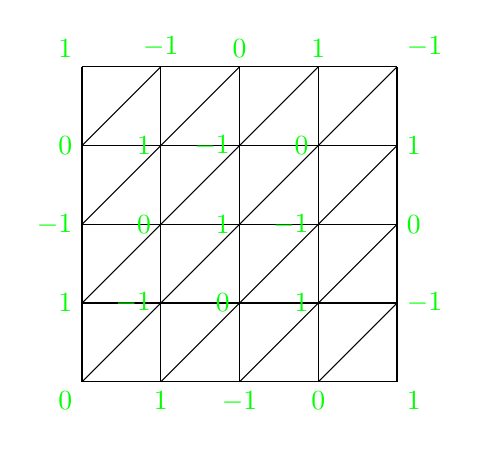
\begin{tikzpicture}
    \draw (0,0) -- (0, 4);
    \draw (1,0) -- (1, 4);
    \draw (2,0) -- (2, 4);
    \draw (3,0) -- (3, 4);
    \draw (4,0) -- (4, 4);

    \draw (0,0) -- (4, 0);
    \draw (0,1) -- (4, 1);
    \draw (0,2) -- (4, 2);
    \draw (0,3) -- (4, 3);
    \draw (0,4) -- (4, 4);

    \draw (0,0) -- (4, 4);
    \draw (0,1) -- (3, 4);
    \draw (0,2) -- (2, 4);
    \draw (0,3) -- (1, 4);
    \draw (1,0) -- (4, 3);
    \draw (2,0) -- (4, 2);
    \draw (3,0) -- (4, 1);
    \draw[color = green] (0, 4) node[above left] {$1$};
    \draw[color = green] (0, 3) node[left] {$0$};
    \draw[color = green] (0, 2) node[left] {$-1$};
    \draw[color = green] (0, 1) node[left] {$1$};
    \draw[color = green] (0, 0) node[below left] {$0$};

    \draw[color = green] (1, 4) node[above] {$-1$};
    \draw[color = green] (1, 3) node[left] {$1$};
    \draw[color = green] (1, 2) node[left] {$0$};
    \draw[color = green] (1, 1) node[left] {$-1$};
    \draw[color = green] (1, 0) node[below] {$1$};


    \draw[color = green] (2, 4) node[above] {$0$};
    \draw[color = green] (2, 3) node[left] {$-1$};
    \draw[color = green] (2, 2) node[left] {$1$};
    \draw[color = green] (2, 1) node[left] {$0$};
    \draw[color = green] (2, 0) node[below] {$-1$};

    \draw[color = green] (3, 4) node[above] {$1$};
    \draw[color = green] (3, 3) node[left] {$0$};
    \draw[color = green] (3, 2) node[left] {$-1$};
    \draw[color = green] (3, 1) node[left] {$1$};
    \draw[color = green] (3, 0) node[below] {$0$};


    \draw[color = green] (4, 4) node[above right] {$-1$};
    \draw[color = green] (4, 3) node[right] {$1$};
    \draw[color = green] (4, 2) node[right] {$0$};
    \draw[color = green] (4, 1) node[right] {$-1$};
    \draw[color = green] (4, 0) node[below right] {$1$};

  \end{tikzpicture}
\hspace{2cm}
  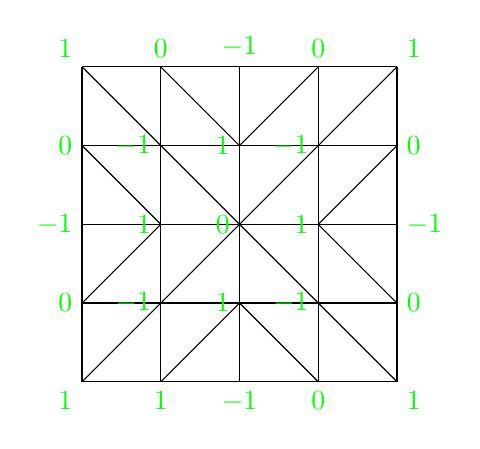
\begin{tikzpicture}
    \draw (0,0) -- (0, 4);
    \draw (1,0) -- (1, 4);
    \draw (2,0) -- (2, 4);
    \draw (3,0) -- (3, 4);
    \draw (4,0) -- (4, 4);

    \draw (0,0) -- (4, 0);
    \draw (0,1) -- (4, 1);
    \draw (0,2) -- (4, 2);
    \draw (0,3) -- (4, 3);
    \draw (0,4) -- (4, 4);

    \draw (0,0) -- (4, 4);
    \draw (0,4) -- (4, 0);

    \draw (0,3) -- (1, 2);
    \draw (1,4) -- (2, 3);

    \draw (0,1) -- (1, 2);
    \draw (1,0) -- (2, 1);

    \draw (3,0) -- (2, 1);
    \draw (4,1) -- (3, 2);

    \draw (2,3) -- (3, 4);
    \draw (3,2) -- (4, 3);

    \draw[color = green] (0, 4) node[above left] {$1$};
    \draw[color = green] (0, 3) node[left] {$0$};
    \draw[color = green] (0, 2) node[left] {$-1$};
    \draw[color = green] (0, 1) node[left] {$0$};
    \draw[color = green] (0, 0) node[below left] {$1$};

    \draw[color = green] (1, 4) node[above] {$0$};
    \draw[color = green] (1, 3) node[left] {$-1$};
    \draw[color = green] (1, 2) node[left] {$1$};
    \draw[color = green] (1, 1) node[left] {$-1$};
    \draw[color = green] (1, 0) node[below] {$1$};


    \draw[color = green] (2, 4) node[above] {$-1$};
    \draw[color = green] (2, 3) node[left] {$1$};
    \draw[color = green] (2, 2) node[left] {$0$};
    \draw[color = green] (2, 1) node[left] {$1$};
    \draw[color = green] (2, 0) node[below] {$-1$};

    \draw[color = green] (3, 4) node[above] {$0$};
    \draw[color = green] (3, 3) node[left] {$-1$};
    \draw[color = green] (3, 2) node[left] {$1$};
    \draw[color = green] (3, 1) node[left] {$-1$};
    \draw[color = green] (3, 0) node[below] {$0$};


    \draw[color = green] (4, 4) node[above right] {$1$};
    \draw[color = green] (4, 3) node[right] {$0$};
    \draw[color = green] (4, 2) node[right] {$-1$};
    \draw[color = green] (4, 1) node[right] {$0$};
    \draw[color = green] (4, 0) node[below right] {$1$};

  \end{tikzpicture}

  \caption{Schachbrettinstabilitäten, $n = 4$}
  \label{fig:schachbrett}
\end{figure}

Diese Druckmoden heißen \markdef{Schachbrettinstabilitäten}. 
\end{beispiel*}
\begin{beispiel} Das $P_{1}-P_{0}$-Element

Die diskrete Inf-Sup-Bedingung erzwingt, dass der diskrete Druckraum genügend klein ist. Für das $P_{1}-P_{1}$-Element gilt das nicht. Beim  $P_{1}-P_{0}$-Element versucht man, dies mit Funktionen niedrigerer Ordnung für den Druck. Für $P_{1}-P_{0}$ gilt $\nabla\cdot[P_{1}]\subset P_{0}$, das heißt, diskret divergenzfreie Funktionen sind divergenzfrei im schwachen Sinn.
\begin{align*}
  u_{h} \in V_{\div}^{h}: \int_{\Omega} (\nabla\cdot u_{h}) q_{h} dx = 0 \quad \forall q_{h} \in Q_{h}\\
q_{h} = \nabla\cdot[P_{1}] \subset P_{0}\\
\implies \int_{\Omega} (\nabla\cdot u_{h})^{2} dx = 0 \implies \nabla\cdot u_{h} = 0
\end{align*}
Das $P_{1}-P_{0}$ Element erfüllt jedoch im Allgemeinen die diskrete Inf-Sup-Bedingung nicht. Auf dem obigen Gitter haben ein $P_{1}$-Druck (25-1) Freiheitsgrade und $P_{0}$ (32-1) Freiheitsgrade. Deshalb sind Druckmoden zu erwarten. Darüberhinaus kann es zu einem sogenannten \emph{Locking} kommen. Um zu zeigen, dass störende Druckmoden (spurious oscillations) auftreten können, betrachten wir ein strukturiertes Gitter vom obigen Typ mit $2n^{2}$ Dreiecken, $n> 1$. Dann
\begin{align*}
\dim V_{h} = 2(n-1)^{2}  
\end{align*}
(Anzahl der inneren Knoten, mit zwei Geschwindigkeitskomponenten). Weiter gilt
\begin{align*}
  Q_{h} = 2n^{2} -1. 
\end{align*}
Es folgt
\begin{align*}
  \dim V_{h} - \dim Q_{h} = \dim V_{\div}^{h} = 2n^{2} - 4n + 2 - 2n^{2} + 1= -4n + 3 < 0, 
\end{align*}
für $n \geq 1$. Folglich ist die notwendige Bedingung $\dim(V_{h}) \geq \dim(Q_{h})$ nicht gegeben. Deshalb sind mindestens $(4n-3)$ Zeilen von $B_{h}$ abhängig. Deshalb gibt es einen Unterraum der Dimension $4n - 3$, sodass für alle $q_{n}$ aus diesem Unterraum gilt $- (\nabla\cdot v_{h}, q_{h})$ für alle $v_{h} \in V_{h}$. Man kann dieses einfache Beispiel auf komplexe Gebiete und Triangulierungen verallgemeinern. 
\end{beispiel}
Nun zum Locking-Phänomen:
Betrachte $\Omega = (0, 1)^{2}$ mit der gezeichneten Triangulierung.
\begin{figure}[h!]
  \centering
  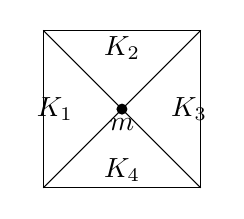
\begin{tikzpicture}
    \draw (0, 0) rectangle (2, 2);
    \draw (2, 2) -- (0, 0);
    \draw (0, 2) -- (2, 0);

    \draw (1, 0.5) node[below] {$K_{4}$};
    \draw (1, 1.5) node[above] {$K_{2}$};
    \draw (0.5, 1) node [left] {$K_{1}$};
    \draw (1.5, 1) node[right] {$K_{3}$};
    \draw (1, 1) node[below] {$m$};
    \fill (1, 1) circle (2pt);
  \end{tikzpicture}
  \caption{Triangulierung}
  \label{fig:tri}
\end{figure}
 Die stückweise konstanten Drücke auf $K_{i}$, $i = 1, \dots, 4$, seien mit $q_{h}^{1}, \dots, q_{h}^{4}$ bezeichnet. 
Aus $q_{h} =  q_{n}^{1} + q_{n}^{2} + q_{n}^{3}+ q_{n}^{4} \in L_{0}^{2} (\Omega_{h}) $  folgt
\begin{align*}
  \int_{\Omega} q_{h} dx = 0 \iff q_{n}^{1} + q_{n}^{2} + q_{n}^{3}+ q_{n}^{4} = 0, 
\end{align*}
da alle Dreiecke $K$ die gleiche Fläche haben. Es gibt also drei unabhängige Druckfreiheitsgrade. Eine Funktion $v_{h} \in V_{\div}^{h}$ muss also drei unabhängige Bedingungen erfüllen. Eine Funtkeion $u_{h} \in V_{h}$ hat jedoch nur zwei unabhängige Freiheitsgrade (im Mittelpunkt des Gitters). 

Sei $v_{h} = (u_{h}^{1}, u_{h}^{2})^{T}$, dann gilt
\begin{align*}
  \nabla\cdot v_{h}|_{K_{1}} &= \frac {u_{h}^{1} (m)} {\frac 12} = - \nabla\cdot v_{h}|_{K_{3}}\\
  \nabla\cdot v_{h}|_{K_{4}} &= \frac {u_{h}^{2} (m)} {\frac 12} = - \nabla\cdot v_{h}|_{K_{2}}. 
\end{align*} 
Falls $v_{h} \in V_{\div}^{h}$ sein soll, muss gelten
\begin{align*}
   0&= ( \nabla\cdot v_{h}, q_{h}) = \norm{K_{1}} (q_{h}^{1} \nabla\cdot v_{h}|_{K_{1}} + q_{h}^{2} \nabla\cdot v_{h}|_{K_{2}} + q_{h}^{3} \nabla\cdot v_{h}|_{K_{3}} + q_{h}^{4} \nabla\cdot v_{h}|_{K_{4}})\\
&=\norm{K_{1}} (2 u_{h}^{1} (m)q_{h}^{1} - 2 u_{h}^{1}(m)q_{h}^{3} - 2 u_{h}^{2}(m) q_{h}^{2} q_{h}^{2} + 2 q_{h}^{2}(m) (- q_{h}^{1} - q_{h}^{2} - q_{h}^{3}))\\
&=\norm{K_{1}} (2 u_{h}^{1} (m)(q_{h}^{1} q_{h}^{3}) - 2 u_{h}^{2}(m)(2q_{h}^{2} + q_{h}^{1} + q_{h}^{3}))
\end{align*}
für beliebige $q_{h}^{1},q_{h}^{2},q_{h}^{3}$. Setze $q_{h}^{1} = 1, q_{h}^{3} = 0$, dann folgt $u_{h}^{2} = 0$. Setze $q_{h}^{3} = 0, q_{h}^{2} = 0$, dann folgt $u_{h}^{1} = u_{h}^{2} = 0$. Schließlich folgt $V_{\div}^{h} = \set 0$.
%\datum{22. Juni 2015}
\begin{beispiel}Das $Q_{1}-Q_{0}$-Element

Sei $\Omega = (0, 1)^{2}$ und eine Triangulierung von $\Omega$ gegeben, die aus $n \times n $ Quadraten besteht, wobei $n$ gerade ist.
\begin{figure}[h!]
  \centering
  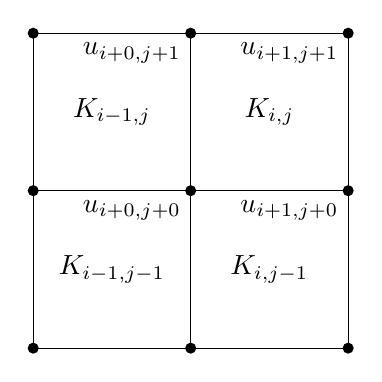
\begin{tikzpicture}[scale = 2]
    \draw (0, 0) rectangle (2, 2);
    \draw (1, 0) -- (1, 2);
    \draw (0, 1) -- (2, 1);  
    \foreach \x in {0,...,2}
    \foreach \y in {0,...,2} 
       {\pgfmathtruncatemacro{\label}{\x - 5 *  \y +21}
       \fill (\x*1, \y*1) circle (1pt);} 
    \foreach \x in {1,...,2}
    \foreach \y in {1,...,2} 
       {\pgfmathtruncatemacro{\i}{\x-1}
        \pgfmathtruncatemacro{\j}{\y-1}
       \draw (\x*1, \y*1) node[below left] {$u_{i+\i, j+\j}$};}
       \draw (0.5 , 0.5) node {$K_{i-1,j-1}$};
       \draw (1.5 , 0.5) node {$K_{i,j-1}$};
       \draw (0.5 , 1.5) node {$K_{i-1,j}$};
       \draw (1.5 , 1.5) node {$K_{i,j}$};

  \end{tikzpicture}
  \caption{Triangulierung des Einheitsquadrates}
  \label{fig:unit_square}
\end{figure}
Die Quadrate werden mit $K_{ij}$ bezeichnet, mit $i, j = 1, \dots, N$. Es wird eine Anordnung von links nach rechts und von oben nach unten benutzt. Die FEM-Geschwindigkeit ist stückweise bilinear und sie wird durch ihre Werte an den Knoten der Quadrate $K_{ij}$ bestimmt.

Bezeichne den Wert am unteren linken Knoten des Quadrats $K_{ij}$ durch $v_{ij}^{h}= (u_{ij}^{1, h}, u_{ij}^{2, h})^{T}$. Eine stückweise Funktion wird benutzt, um den Druck zu approximieren. Im Vergleich zum $P_{1}- P_{0}$-Element auf einem entsprechenden Gitter werden die Quadrate hier durch ihre Diegonalen nicht geteilt. Hierbei ist die Anzahl der Geschwindeigkeitsfreiheitsgrade von $P_{1}-P_{0}$ und $Q_{1}-Q_{0}$ dieselbe, da die Zahl der inneren Knoten die gleiche ist. Die Druckfreiheitsgrade sind jedoch nur ungefähr halb so viele (Anzahl der Zahlen -1). Die Inf-Sup-Stabilität von $Q_{1}-Q_{0}$ gegenüber $P_{1} - P_{0}$ ist somit zumindest denkbar. Da der Mittelwert der diskreten FEM-Drücke $0$ ist, folgt
\begin{align*}
  0 &= \int_{\Omega} q_{h} dx\\
  & = \sum_{i, j = 1}^{n} \int_{K_{ij}} q_{ij}^{h} dx\\
  &= h^{2} \sum_{i, j = 1}^{n} q_{ij}^{h},
\end{align*}
wobei $h$ die Seitenlänge der $K_{ij}$ ist. Wir erhalten
\begin{align*}
  \sum_{i, j = 0}^{n} q_{ij}^{h} = 0.
\end{align*}
Wir betrachten nun eine einzelne Gitterzelle $K_{ij}$: Partielle Integration ergibt
\begin{align*}
  \int_{K_{ij}} \nabla\cdot q_{ij}^{h} dx  &= q_{ij}^{h} \int_{K_{ij}} \nabla\cdot v_{h} dx\\
  &= q_{ij}^{h} \int_{\partial K_{ij}} v_{h}\cdot n_{\partial K_{ij}} dx,
\end{align*}
wobei $v_{h} = (u^{1, h}, u^{2, h})^{T}$ und $n_{\partial K_{ij}}$ die äußere Einheitnormale bezeichnet. Die Einheitsnormalen sind $\partial K_{ij} \pm e_{i}$, $i = 1, 2$. Das Kantenintegral über die Restriktion von $Q_{1}$ auf eine Kante ist eine lineare Funktion, die mit der Trapezregel exakt berechnet werden können. Man erhält zum Beispiel für die unterste Kante
\begin{align*}
  \int_{E} v_{h}\cdot n_{\partial K_{ij}} dx = -\int_{E} v_{h} e_{2} dx =  - \int_{E} u^{2, h}(x) dx = -\frac h 2 (u_{i, j}^{2, h} + u_{i+1, j}^{2, h}). 
\end{align*}
Zusammen gilt also
\begin{align*}
  \int_{K_{ij}} (\nabla\cdot v_{h})q^{h} dx = \frac h 2 q_{ij}^{h}(- u_{i,j}^{2, h} - u_{i+1, j}^{2, h} + u_{i+1, j}^{1, h}+ u_{i+1, j+1}^{1, h} + u_{i+1, j+1}^{2, h} + u_{1, j+1}^{2, h} - u_{i, j+1}^{1, h} - u_{i, j}^{1, h})
\end{align*}
Man betrachtet nun die Beiträge der Integrale, die mit einem inneren Geschwindigkeitsknoten verbunden sind. Man erhält für die Knoten $ij$, $i, j = 2, \dots, n$ die folgenden Beiträge von den vier Gitterzellen, die min dem Knoten adjazent sind:
\begin{align*}
  u_{i, j}^{1, h}\frac h 2 (q_{i-1, j-1}^{h} + q_{i-1, j}^{h} - q_{i, j-1}^{h} - q_{i, j}^{h}) + 
  u_{i, j}^{2, h}\frac h 2 (q_{i-1, j-1}^{h} + q_{i, j-1}^{h} - q_{i-1, j}^{h} - q_{i, j}^{h}).
\end{align*}
Die Summe der Integrale über die Gitterzellen ist die gleiche wie die der Gebiete, die mit einem inneren Knoten verbunden sind.
\begin{align*}
  0 &= (\nabla\cdot v_{h}, \phi_{h})= \sum_{i, j = 1}^{n} (\nabla\cdot v_{h}, q_{h})_{K_{ij}} \\
&= \frac h 2 \int_{i, j = 2}^{n}\(  u_{i, j}^{1, h} (q_{i-1, j-1}^{h} + q_{i-1, j}^{h} - q_{i, j-1}^{h} - q_{i, j}^{h}) +   u_{i, j}^{2, h}(q_{i-1, j-1}^{h} + q_{i, j-1}^{h} - q_{i-1, j}^{h} - q_{i, j}^{h})\)
\end{align*}
Insbesondere gilt diese Gleichheit für alle diskreten Geschwindigkeiten, in denen nur ein Wert $u_{i, j}^{1, h}$ oder $u_{i, j}^{2, h}$  nicht $0$ ist. Um eine Druckmode zu konstruieren, setzt man ein $u_{i, j}^{1, h}$ und $u_{i, j}^{2, h}$ auf $0$ und erhält
\begin{align*}
 & q_{i-1, j-1}^{h} + q_{i-1, j}^{h} - q_{i, j-1}^{h} - q_{i, j}^{h}= 0\\
 & q_{i-1, j-1}^{h} + q_{i, j-1}^{h} - q_{i-1, j}^{h} - q_{i, j}^{h}= 0
\end{align*}
Addieren und Subtrahieren der Bedingungen ergibt
\begin{align*}
  &q_{i-1, j-1}^{n} = q_{i, j}^{h},\\
  &q_{i-1, j}^{n} = q_{i-1, j}^{h}, \quad i, j = 2, \dots, n. 
\end{align*}
Damit gibt es auf den ersten Blick zwei Freiheitsgrade, die wählbar sind, um einen Druckmode zu konstruieren. Wenn man zum Beispiel $q_{11} = \alpha \in \R$, $\alpha \neq 0$ setzt, so hat die Hälfte der Gitterzellen den gleichen Wert, nämlich überall, wo die Summe der Indizes $i + j$  von $q_{ij}$ gerade ist. Indem man zum Beispiel $q_{21} \coloneqq \beta$ setzt, erhält man die andere Hälfte der Gitterzellen ihren Druckwert. Hier geht die Annahme ein, dass $n$ gerade gewählt war. Aus $q_{h} \in L_{0}^{2}(\Omega)$ folgt
\begin{align*}
  0 = \sum_{i, j = 1, i+j \mod 2 = 0}^{n} \alpha n^{2} + \sum_{i, j = 1, i+1 mod 2 = 1}^{n} \beta n^{2} = \frac {n^{2}} 2 (\alpha + \beta)n^{2} \implies \beta = -\alpha. 
\end{align*}
Für alle $\alpha \neq 0$ würde eine Druckmode konstruiert, sodass $(\nabla\cdot v_{h}, v_{h}) = 0$ für alle $v_{h} \in V_{h}$.
\begin{figure}[h!]
  \centering
  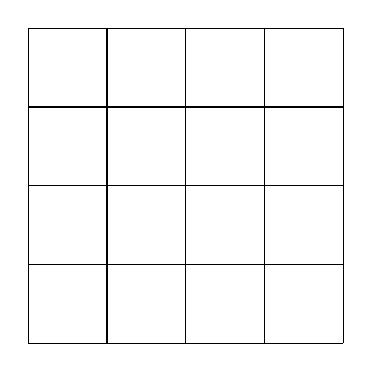
\begin{tikzpicture}

    \foreach \y in {0,...,4} 
    {       \draw (0, \y) -- (4, \y);
      \draw ( \y, 0) -- (\y, 4);}

    \foreach \y in {1, \dots, 4}
    \foreach \x in {1, 2}
%    { \pgfmathifthenelse {\x\y < 0}{\draw (\y - 0.5, \x-0.5) node{1}}{\draw (\y - 0.5, \x-0.5) node{1}};}
{}
  \end{tikzpicture}
  \caption{Schachbrett-Instabilität}
  \label{fig:schachbrett-2}
\end{figure}
\end{beispiel}
\begin{bemerkung*}
  \begin{enumerate}
  \item Konstruiert man fpr das $Q_{1}- Q_{0}$-Element einen rdigierten Druckraum $\tilde Q_{h} = \set{\rho_{h}}^{\perp}$, dann hat $Q_{1}- \tilde Q_{h}$-Element eine Inf-Sup-Konstante $\beta_{h}= \cO(h)$. 
\item Durch Entfernen weiterer diskreter Drücke erhält man ein Inf-Sup-stabiles Element zu (i). 
  \end{enumerate}
\end{bemerkung*}
\begin{lemma} Aublin-Nitsche-Lemma
  
Es werde $g \in L^{2}(\Omega)$ die eindeutige Lösung $\phi_{g} \in H_{0}^{1}(\Omega)$ zugeordnet, die
\begin{align*}
  (\nabla w, \nabla \phi_{g}) = (g, w) 
\end{align*}
für alle $w \in H_{0}^{1}(\Omega)$ erfüllt. Sei nun $u  \in H_{0}^{1}(\Omega)$ die Lösung von
\begin{align*}
(\nabla u, \nabla v) = (f, v), \quad \forall v \in H_{0}^{1}(\Omega)
\end{align*}
mit $f \in L^{2}(\Omega)$ und sei $u_{h} \in V_{h} \subset H_{0}^{1} (\Omega)$ die diskrete Lösung von 
\begin{align*}
  (\nabla u_{h}, \nabla v_{h}) = (f, v_{h}), \quad \forall v_{h} \in V_{h}.
\end{align*}
Dann gilt
\begin{align*}
  \nnorm{u- u_{h}}_{L^{2}} \leq C \cdot \nnorm{\nabla u - \nabla u_{h}}_{L^{2}}\cdot \sup_{0 \neq g \in L^{2}(\Omega)}\set{\frac 1 {\nnorm g_{L^{2}}}\nnorm{inf_{v_{h} \in V_{h}} \nnorm{\nabla \phi_{g} - \nabla v_{h}}_{L^{2}}}}. 
\end{align*}
\end{lemma}
\begin{beweis}
  Es gilt für $w = u - u_{h} \in L^{2}(\Omega)$:
  \begin{align*}
    \nnorm w_{L^{2}} = \sup_{0 \neq g \in L^{2}(\Omega)} \frac{(g, w)}{\nnorm{g}_{L^{2}}}. 
  \end{align*}
Aus $(\nabla u - \nabla u_{h}, \nabla \phi_{g}) = (g, w)$ folgt für $w = u - u_{h}$
\begin{align*}
  &(\nabla u - \nabla u_{h}, \nabla \phi_{g})= (g, u- u_{h})\\
  &(\nabla u - \nabla u_{h}, \nabla \phi_{g} - \nabla v_{h}) \leq \nnorm {\nabla u - \nabla u_{h}}_{L^{2}} \cdot \nnorm{\nabla \phi_{g} - \nabla v_{h}}_{L^{2}}\\
\implies & (g, u - u_{h}) \leq \nnorm{\nabla u - \nabla u_{h}}_{L^{2}} \cdot \inf_{v_{h}\in V_{h}} \nnorm{\nabla \phi_{g} - \nabla v_{h}}_{L^{2}}
\end{align*}
Dieses Dualitätsargument liefert nun
\begin{align*}
  \nnorm{u - u_{h}}_{L^{2}}&\leq \sup_{0 \neq g \in L^{2}} \frac{g, u - u_{h}}{ \nnorm g_{L^{2}}}\\
&\leq \nnorm{\nabla u - \nabla u_{h}}_{L^{2}} \cdot \sup_{0 \neq g \in L^{2}} \inf_{v_{h} \in V_{h}} \frac{\nnorm{\nabla \phi_{g} - \nabla v_{h}}_{L^{2}}}{\nnorm g_{L^{2}}}. 
\end{align*}
\end{beweis}
%\datum{24. Juni 2015}

\begin{folgerung}
  Sei $\Omega$ konvex. Dann $\phi_{g} \in H^{2}(\Omega)$, $\norm{\phi_{g}}_{2}\leq C_{\Omega} \cdot \nnorm{g}_{L^{2}}$
  \begin{enumerate}
  \item Sei $u \in H^{1}(\Omega)$. Dann
    \begin{align*}
      \nnorm{u-u_{h}}_{L^{2}} &\leq \nnorm{u-u_{h}}_{V} \cdot \sup_{0 \neq g \in L^{2}} \frac {1}{\nnorm{g}_{L^{2}}}\inf_{v_{h} \in V_{h}} \underbrace{\nnorm{\phi_{g} - v_{h}}_{V}}_{= C\cdot h\cdot \nnorm{\phi_{g}}_{2}} \leq C \cdot C_{\Omega}\cdot h\cdot \nnorm{g}_{L^{2}}\\
&\leq \nnorm{u-u_{h}}_{V}\cdot C \cdot C_{\Omega}\cdot h
    \end{align*}
\item Sei $u \in H^{2} (\Omega)$.
  \begin{align*}
      \nnorm{u-u_{h}}_{L^{2}} &\leq \underbrace{\nnorm{u-u_{h}}_{V}}_{\leq C\cdot h\cdot \norm 2_{2}}  \cdot C\cdot C_{\Omega} \cdot h \leq C' h^{2} \norm u _{2} \leq C''\cdot h^{2}\cdot \nnorm f_{L^{2}}. 
  \end{align*}
\end{enumerate}
\end{folgerung}

\paragraph{Das Minielement}
\label{sec:das-minielement}

Typisch für das Minielement ist, dass der Raum $X_{h}$ für die Geschwindigkeit durch die Hinzunahme von Bubblefunktionen genügend groß wird. Seien $\lambda_{1}, \lambda_{2}, \lambda_{3}$ baryzentrische Koordinaten, die im Einheitsdreieck mit $x_{1}, x_{2}$ und $(1- x_{2} - 1_{1})$ zusammenfallen. Dann verschwindet $b(x) = \lambda_{1}\cdot \lambda_{2}\cdot \lambda_{3}$ auf den Seiten des Dreiecks. In 3D auf einem Tetraeder wählt man
\begin{align*}
  b(x) = \lambda_{1}\cdot \lambda_{2}\cdot \lambda_{3}\cdot \lambda_{4}. 
\end{align*}
Die Hinzunahme einer solchen Bubble zum Geschwindigkeitsraum $P_{1}$ ändert die Stetigkeit nicht. 
\begin{figure}[h!]
  \centering
  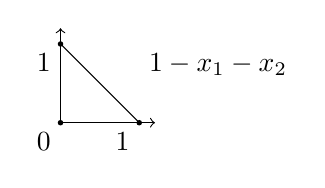
\begin{tikzpicture}
      \draw[->] (0,0) -- coordinate (x axis mid) (1.2,0);
      \draw[->] (0,0) -- coordinate (y axis mid) (0,1.2);
      \draw (1, 0) -- (0, 1);
      \fill (0,0) circle (1pt) node[below left] {$0$};
      \fill (0,1) circle (1pt) node[below left] {$1$};
      \fill (1,0) circle (1pt) node[below left] {$1$};
      \fill (3, 1)  node[below left] {$1- x_{1}-x_{2}$};
  \end{tikzpicture}
  \caption{Mini}
  \label{fig:mini}
\end{figure}
$V_{h} = (P_{1} + B_{h})^{2}, \, Q_{h} = P_{1} \cap L_{0}^{2}(\Omega)$ (in 3D: $V_{h}=(P_{1} + B_{h})^{3}$), mit
\begin{align*}
  B_{h} &= \set{v \in C_{0}(\bar \Omega): v_{T} \in \Span{\lambda_{1}, \lambda_{2}, \lambda_{3}}, \, T \in \cT_{h}}\\
  B_{h} &= \set{v \in C_{0}(\bar \Omega): v_{T} \in \Span{\lambda_{1}, \lambda_{2}, \lambda_{3}, \lambda_{4}}, \, T \in \cT_{h}}
\end{align*}
(2D/3D). Da der Träger jeder Bubble auf ein einziges Element beschränkt ist, können alle Bubbles durch statische Kondensation eleminiert werden. 
Das Minielement ist eines der am wenigesten aufwendigen Elemente.
\begin{satz}
  Sei $\Omega$ konvex. Dann erfüllt das Minielement dauf quasiuniformen Triangulierungen $\cT_{h}$ die Inf-Sup-Bedinung mit einem $\beta > 0$. 
\end{satz}
\begin{beweis}
Zur Anwendung von Fortins Kriterium definiert man zunächst einen Projektor $\Pi_{h}^{0}: H_{0}^{1}(\Omega) \to P_{1}(\cT_{h})$ über die Lösung der Helmholtzgleichungen
\begin{align*}
  (\nabla(\Pi_{h}^{0}v), \nabla w_{h}) + (\Pi_{h}^{0}(v), w_{h}) = (\nabla u, \nabla w_{h}) + (v, w_{h})\quad w_{h}\in P_{1}(\cT_{h}).
\end{align*}
Offensichtlich gilt
\begin{align*}
  \nnorm{\Pi_{h}^{0}v}_{1} \leq \nnorm v_{1}
\end{align*}
für alle $v \in H^{1}(\Omega)$. Das Dualitätsargument auf einem konvexen Gebiet liefert
\begin{align*}
  \nnorm{\Pi_{h}^{0}v - v}_{0} &\leq C_{1}\cdot h \cdot \nnorm{\Pi_{h}^{0} v - v}_{1}\\
&\leq C_{1}\cdot h \cdot\(\nnorm{\Pi_{0}^{h} v}_{1} + \nnorm v _{1}\) \\
&\leq C_{2}\cdot h \cdot \nnorm v _{1}
\end{align*}
(wichtige Eigenschaft!)  
Weiterhin definieren wir eine lineare Abbildung $\Pi_{h}^{1}: L_{2}(\Omega) \to B_{h}$ mit
\begin{align*}
  \int_{T}(\Pi_{h}^{1}v - v)dx = 0, \quad \forall T \in \cT_{h}. 
\end{align*}
Die Abbildung besteht aus einem zweistufigen Prozess. Zunächst erfolgt die $L^{2}$-Projektion auf die stückweise konstanten Funktionen. Anschließend werden die konstanten Funktionen durch Bubble-Funktionen mit dem gleichen Integral ersetzt. Dann erhält man $\nnorm{\Pi_{h}^{1} v}_{0} \leq C_{3}\cdot \nnorm v _{0}$. 

\paragraph{$L_{2}$-Stabilität von $\Pi_{h}^{1}v$:}
\label{sec:l_2-stabilitat-von}



\begin{enumerate}
\item Mit $w_{i} > 0$, $\sum_{i = 1}^{N_{0}} w_{i} = 1$. 
  \begin{align*}
    \norm{\int_{T} b \, dx} &= \norm T \cdot\norm {\sum_{i = 0}^{N_{0}} w_{i} b(x_{1})}\\
    &= \norm T \( \min_{1, \dots, N_{0}} b(x_{i})\) \sum_{i = 0}^{N_{0}} w_{i}\\
    &= C\cdot\norm T
  \end{align*}
(2D: $C \geq \frac 1 {10}$, 3D: $C \geq \frac 1 {100}$). Wir setzen jetzt
\begin{align*}
  \lambda\int_{T} b \, dx = \int_{T} v \, dx \implies \norm{\int_{T} v dx} \geq \lambda\cdot C\cdot \norm T. \\
\implies\quad \lambda \leq \frac 1 C \norm T^{-1} \norm{\int_{T} v \, dx}. 
\end{align*}
\item
  \begin{align*}
    \nnorm{b}_{L^{2}(T)} &= \(\int_{T}(\lambda b )^{2}\)^{\frac 12} = \lambda \(\int_{T}b\cdot b \, dx\)^{2}\\
&\leq \lambda\cdot\(\nnorm b_{L^{1}(T)} \cdot \nnorm b_{L^{\infty}(T)}  \)^{\frac 12}\\
&\leq\frac 1 C \norm T^{-1} \nnorm v_{L^{1}(T)}\cdot\(\underbrace{\nnorm b_{L^{1}(T)}}_{\leq \norm T \cdot \nnorm b_{L^{\infty}(T)}} \cdot \nnorm b_{L^{\infty}(T)}  \)^{\frac 12}\\
&\leq\frac 1 C \norm T^{-1} \nnorm v_{L^{1}(T)}\cdot\ \norm T^{\frac 12} \nnorm b_{L^{\infty}(T)}\\
&\leq\frac 1 C \norm T^{-1} \norm T^{\frac 12} \nnorm v_{L^{2}(T)}\cdot\ \norm T^{\frac 12} \nnorm b_{L^{\infty}(T)}\\
&\leq\frac 1 C \cdot\nnorm v_{L^{2}(T)}\cdot \nnorm b_{L^{\infty}}
  \end{align*}
(2D: $\nnorm b_{L^{\infty}} = \frac 1 {27}$, 3D: $\nnorm b_{L^{\infty}} = \frac 1 {256}$) Ausflug endet. 

\vspace{5mm}
Setzt man nun
\begin{align*}
  \Pi_{h} v \coloneqq \Pi_{h}^{0}v + \Pi_{h}^{1}(v - \Pi_{h}^{0} v),
\end{align*}
so gilt
\begin{align*}
  \int_{T}(\Pi_{h}v - v) dx &=   \int_{T}\Pi^{0}_{h}v  dx +  \int_{T}\Pi^{1}_{h}(v - \Pi_{h}^{0} v )dx - \int_{T} v \; dx\\
&=   \int_{T}\Pi^{0}_{h}v  dx +  \int_{T}(v - \Pi^{0}_{h})dx - \int_{T} v \; dx = 0. 
\end{align*}
Die Definition der Abbildung $\Pi_{h}$ wird nun komponentenweise auf vektorwertige Funktionen angewendet. Man beachte, dass die Gradienten der Drücke stückweise konstant sind und die Stetigkeit zu erfolgen hat:
\begin{align*}
  \int_{\Omega} \nabla\cdot(v - \Pi_{h}v) q_{h} \, dx &= \int_{\partial \Omega} \underbrace{(v - \Pi_{h}v)}_{= 0}\cdot n q_{h} ds - \int_{\Omega}\underbrace{(v - \Pi_{h} v)}_{= 0}\nabla q_{h}\, dx = 0. 
\end{align*}
Weiterhin gilt
\begin{align*}
  \nnorm{\Pi_{h}v}_{1} &\leq   \nnorm{\Pi^{0}_{h}v}_{1} +   \nnorm{\Pi_{h}^{1}(v- \Pi_{h}^{0}v)} _{1}\\
&\leq   \nnorm{v}_{1} +   C_{inv} h^{-1} \nnorm{\Pi_{h}^{1}(v- \Pi_{h}^{0}v)} _{0}\\
&\leq   \nnorm{v}_{1} +   C_{inv} \cdot C_{3} \cdot h^{-1} \nnorm{v- \Pi_{h}^{0}v} _{0}\\
&\leq   \nnorm{v}_{1} +   C_{inv} \cdot C_{3} \cdot h^{-1}\cdot C_{2}\cdot h \nnorm{v} _{0}\\
&\leq  (1+  C_{inv} \cdot C_{3} \cdot C_{2}) \nnorm{v} _{1}
\end{align*}
\end{enumerate}
Damit ist die Beschränktheit von $\Pi_{h}v$ bewiesen und das Minielement ist auf quasi-uniformen Gebieten und konvexen Gebieten $\Omega$ Inf-Sup-stabil. 
\end{beweis}

\paragraph{Minielement $P_1^+-P_1$}
Fehler beträgt bei $u \in H^{2}, p \in H^{1}$ oder $p \in H^{2}$ $\cO(h)$ ('ziemlich verwandt mit $P_{1}-P_{1}$-Stabilisierung'). Es gilt
\begin{align*}
  \nnorm{u -u_{h}}_{V} &\leq 2(1 + C_{F}) \inf_{v_{h} \in V_{h}} \nnorm{u-u_{h}} + \frac 1 \nu \inf_{q_{h}\in Q} \nnorm{p-q_{h}}_{Q}\\
&  \leq 2(1 + C_{F})C_{u} \cdot h\cdot \norm u_{2} + \frac 1 \nu C_{p}\norm p_{1}\cdot h\\
&  \leq 2(1 + C_{F})C_{u} \cdot h\cdot \norm u_{2} + \frac 1 \nu C'_{p}\norm p_{2}\cdot h^{2}
\end{align*}
\begin{bemerkung} Der Boland-Nealandes-Ansatz zur Überprüfung der Inf-Sup-Bedingung. 

Es wird weiter die Konstruktion von FEM-Räumen ($V_{h}, Q_{h}$) betrachtet, die uniform eine Inf-Sup-Bedingung erfüllen. Die Idee von Boland und Nicolaidas besteht darin, das Problem in lokale Inf-Sup-Bedingungen und eine globale, einfachere Inf-Sup-Bedingung zu zerlegen. Sei $\Omega$ dazu partitioniert in eine endliche Zahl $R$ von disjunkten, Lipschitzstetigen, offenen Teilmengen $\Omega_{r}$ mit Rand $\Gamma_{r}$:
\begin{align*}
  \bar \Omega = \bigcup_{r = 1}^{R} \bar \Omega_{r}. 
\end{align*}
Sei weiter $Q_{h}^{+} = Q_{L} \oplus \R$. Für $1 \leq r \leq R$ setzt man
\begin{align*}
  \begin{cases}
    V_{h}(\Omega_{r}) = \set{v \in V_{h}: \, v_{h} = 0 \text{ in } \Omega\setminus \Omega_{r}}\\
    Q_{h}^{+}(\Omega_{r}) = \set{q_{h}|_{\Omega_{r}}: \, q_{h} \in Q_{h}^{+}}\\
    Q_{h}(\Omega_{r}) = Q_{h}^{+}(\Omega_{r})\cap L_{0}^{2}(\Omega_{r}). 
  \end{cases}
\end{align*}
Weiter sei $\bar M_{h}= \set{q_{h} \in L_{0}^{2}(\Omega): q_{h}|_{\Omega_{r}} \text{ ist konstant }, 1 \leq r \leq R}$. Man beachte, dass alle Funktionen aus $V_{h}(\Omega_{r})$ zu $H_{0}^{1}(\Omega_{r})^{d}$ gehören. Nun wird folgende Annahme eingeführt, die auf uniform gültigen lokalen Inf-Sup-Bedingungen bezüglich dieser Partition beruht. 
\end{bemerkung}
\begin{voraussetzung}\label{2.28}
  Es existiere eine Konstante $\lambda^{*} > 0$, die unabhängig von $h$ und $v$ ist, so dass gilt:
  \begin{align*}
    \sup_{v_{h}\in V_{h}(\Omega_{r})} \frac{\int q_{h} (\nabla\cdot v_{h}) dx}{ \nnorm{v_{h}}_{1, \Omega_{r}}} \geq \lambda^{*} \nnorm{q_{h}}_{0, \Omega_{r}}\qquad \forall q_{h} \in Q_{h}(\Omega_{r}), \, 1 \leq r\leq R
  \end{align*}
\end{voraussetzung}
\begin{satz}
  Wenn die Räume $(V_{h}, Q_{h})$ die Voraussetzung \ref{2.28} erfüllen und wenn es einen Teilraum $\bar V_{h}$ von $V_{h}$ gibt, sodass $(\bar V_{h}, \bar M_{h})$ die Inf-Sup-Bedingung mit einer Konstanten $\bar \beta$ unabhängig von $h$ erfüllt, dann erfüllt $(V_{h}, Q_{h})$ ebenfalls die Inf-Sup-Bedingung mit einer Konstanten $\beta^{*}$ unabhängig von $h$. 
\end{satz}
\begin{beweis}
  Jede Funktion $q_{h} \in Q_{h}$ kann dargestellt werden als 
  \begin{align*}
    q_{h} = \tilde q_{h} + \bar q_{h}
  \end{align*}
mit $\bar q_{h}|_{\Omega_{r}} = \frac 1 {\norm{\Omega_{r}}} \int_{\Omega_{r}} q_{h} dx$, $1 \leq r\leq R$, und $\tilde q_{h} = \tilde q_{h}|_{\Omega_{r}} \in Q_{h}^{+}(\Omega_{r})$. Es gilt $\bar q_{h} \in \bar M_{h}$ und die Orthogonalität der Zerlegung impliziert
\begin{align*}
  \nnorm {q_{h}}_{0}^{2} = \nnorm {\tilde q_{h}}_{0}^{2} + \nnorm{\bar q_{h}}^{2}. 
\end{align*}

\end{beweis}


%%% Local Variables: 
%%% mode: latex
%%% TeX-master: "vorlesung"
%%% End: 
